\documentclass[a4paper,13pt]{extreport}
\usepackage{graphicx}
\usepackage{indentfirst}
\usepackage{mathptmx}
\usepackage{amsmath,amsfonts,amssymb,fancyhdr}
\usepackage{amsthm,amsxtra,latexsym, amscd}
\usepackage[utf8]{vietnam}
%\usepackage[unicode,colorlinks=true]{hyperref} 
%\usepackage[utf8]{inputenc}
\usepackage[left=3.50cm, right=2.00cm, top=3.00cm, bottom=3.50cm]{geometry}
\usepackage{tocloft}
\usepackage{type1cm}
\usepackage{vector}
\usepackage{color}
\usepackage[usenames,dvipsnames]{xcolor}
\usepackage{caption/subcaption}
\usepackage[section]{placeins}
%\usepackage{subfigure}
\usepackage{pbox}
%\usepackage[unicode,colorlinks=true]{hyperref}
\usepackage{framed}
\usepackage{multirow}
\usepackage{longtable}

\usepackage[hyphens]{url}
%\usepackage[hidelinks]{hyperref}

\usepackage[ unicode, plainpages = false, pdfpagelabels, 
                 pdfpagelayout = OneColumn, % display single page, advancing flips the page - Sasa Tomic
                 bookmarks = true,
                 bookmarksopen = true,
                 bookmarksnumbered = true,
                 breaklinks = true,
                 linktocpage = false,
                 colorlinks = true,
                 linkcolor = black,
                 urlcolor  = blue,
                 citecolor = black,
                 anchorcolor = green,
                 hyperindex = true,
                 hyperfigures = true,
                 ]{hyperref} 

\usepackage{listings}

\definecolor{dkgreen}{rgb}{0,0.6,0}
\definecolor{gray}{rgb}{0.5,0.5,0.5}
\definecolor{mauve}{rgb}{0.58,0,0.82}

\lstset{frame=single,
		  language=Python,
		  aboveskip=3mm,
		  belowskip=3mm,
		  showstringspaces=false,
		  columns=flexible,
		  basicstyle={\small\ttfamily},
		  numbers=none,
		  numberstyle=\tiny\color{gray},
		  keywordstyle=\color{blue},
		  commentstyle=\color{dkgreen},
		  stringstyle=\color{mauve},
		  breaklines=true,
		  breakatwhitespace=false,
		  tabsize=3
}
%\usepackage{algorithm2e}
\usepackage[chapter]{algorithm}
\usepackage{algpseudocode}
\usepackage{setspace}
\makeatletter
\newcommand{\newalgname}[1]{%
  \renewcommand{\ALG@name}{#1}%
}
\usepackage{longtable}
\usepackage[acronym]{glossaries}
\usepackage{multicol}
\setlength{\columnsep}{25pt}
\usepackage{nomencl}
\makenomenclature

\usepackage{pdfpages}

\usepackage{tabularx}
\captionsetup{compatibility=false}
\renewcommand\cftchappresnum{\chaptername\space}
\setlength{\cftchapnumwidth}{2.5cm}
\usepackage{titlesec}

\usepackage{etoolbox}

\makeatletter
\patchcmd{\ttlh@hang}{\parindent\z@}{\parindent\z@\leavevmode}{}{}
\patchcmd{\ttlh@hang}{\noindent}{}{}{}
\makeatother

\titleformat{\chapter}[display]
  {\normalfont\large\bfseries\centering}{\chaptertitlename\ \thechapter}{20pt}{\huge}
\linespread{1.3}

%\baselineskip 19.5 pt
                 
\begin{document}


\includepdf{docs/BiaChinh}

\includepdf{docs/BiaPhu}
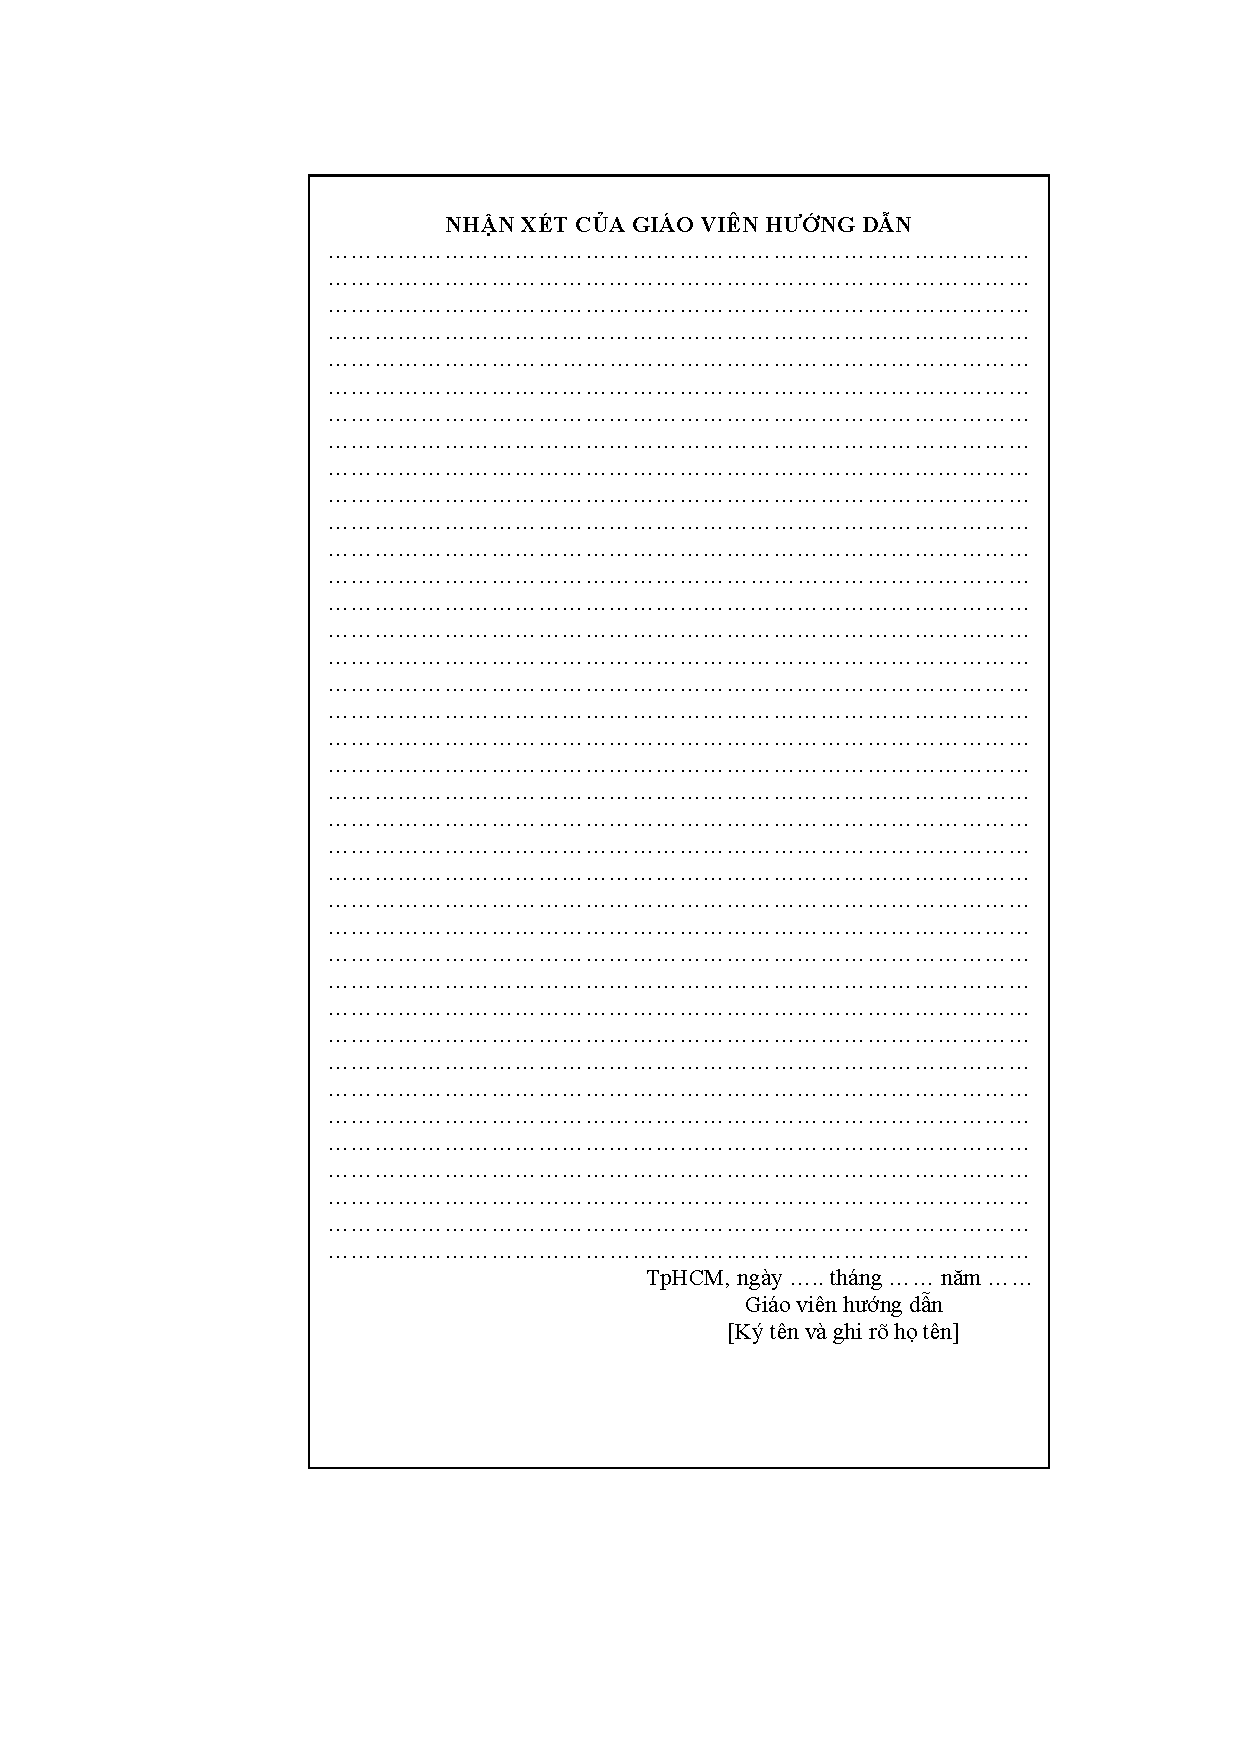
\includepdf[pages=1-2]{docs/NhanXet}

\pagenumbering{roman}
\newpage
\chapter*{LỜI CẢM ƠN}
\addcontentsline{toc}{chapter}{LỜI CẢM ƠN}
%\hspace{0.3in}
Trước tiên, chúng em xin gửi lời tri ân sâu sắc đến Thầy Ngô Minh Nhựt. Thầy đã rất tận tâm, nhiệt tình hướng dẫn và chỉ bảo em trong suốt quá trình thực hiện luận văn. Không có sự quan tâm, theo dõi chặt chẽ của Thầy chắc chắn em không thể hoàn thành luận văn này.

Em xin chân thành cảm ơn quý Thầy Cô khoa Công Nghệ Thông Tin - trường đại học Khoa Học Tự Nhiên, những người đã ân cần giảng dạy, xây dựng cho em một nền tảng kiến thức vững chắc. 

Cuối cùng, chúng con xin cảm ơn ba mẹ đã sinh thành, nuôi dưỡng, và dạy dỗ để chúng con có được thành quả như ngày hôm nay. Ba mẹ luôn là nguồn động viên, nguồn sức mạnh hết sức lớn lao mỗi khi chúng con gặp khó khăn trong cuộc sống.

\hfill TP. Hồ Chí Minh, 7/2017

\hfill \textit{Bùi Trung Hải}

\hfill \textit{Phạm Ngọc Tuấn}


%\newpage
%\thispagestyle{empty}
%\mbox{}

\newpage
\addcontentsline{toc}{chapter}{ĐỀ CƯƠNG CHI TIẾT}
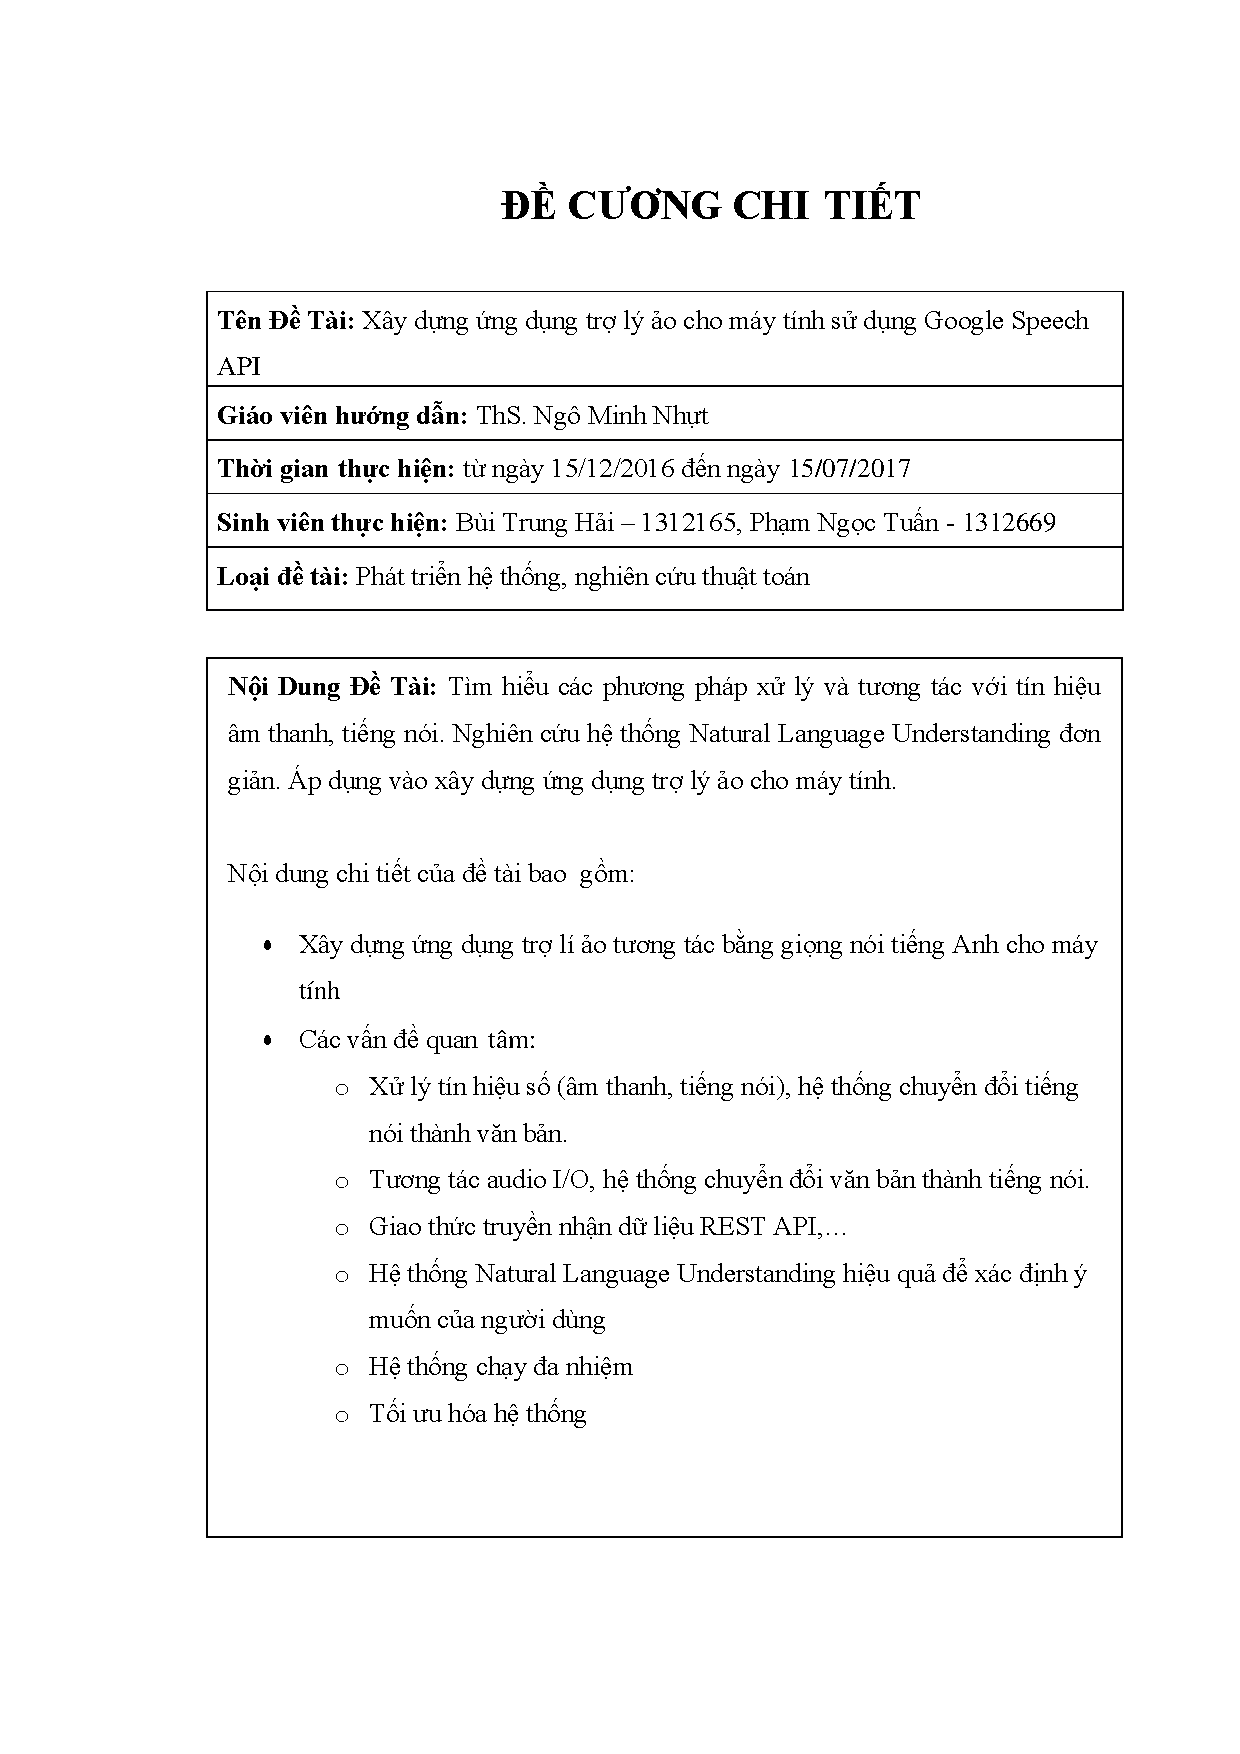
\includepdf[pages=1-3,pagecommand=\thispagestyle{plain}]{docs/DeCuongChiTiet}

\newpage
\renewcommand{\contentsname}{\centerline{MỤC LỤC}}
\addcontentsline{toc}{chapter}{MỤC LỤC}
\tableofcontents

\newpage
\renewcommand\listfigurename{\centerline{DANH MỤC HÌNH ẢNH}}
\addcontentsline{toc}{chapter}{DANH MỤC HÌNH ẢNH}
\listoffigures


\newpage
\renewcommand\listtablename{\centerline{DANH MỤC BẢNG}}
\addcontentsline{toc}{chapter}{DANH MỤC BẢNG}
\listoftables

\newpage
\chapter*{TÓM TẮT KHÓA LUẬN}
\addcontentsline{toc}{chapter}{TÓM TẮT KHÓA LUẬN} 

Trong xu hướng công nghệ hiện nay, vai trò của các trợ lý ảo ngày càng trở nên quan trọng. Các hãng công nghệ lớn thay nhau tung ra những trợ lý ảo của riêng mình tích hợp trên các thiết bị di động: Siri của Apple, Cortana của Microsoft, Google Assistant của Google, Alexa của Amazon,... Chức năng của các trợ lý ảo này ngày càng được mở rộng, từ những chức năng đơn giản như tra cứu, hỏi đáp, đến những chức năng cao hơn như quản lý lịch, gọi điện thoại, dẫn đường, điều khiển các thiết bị khác,... Khóa luận này có mục đích tạo ra một trợ lý ảo có khả năng chạy được trên nhiều nền tảng hệ điều hành khác nhau trên máy tính cá nhân. 

Nhận diện giọng nói là một trong những thành phần quan trọng nhất của một trợ lý ảo. Nhiều công ty và nhóm nghiên cứu lớn nhỏ đã nghiên cứu và đưa ra các bộ toolkit cũng như API cho việc nhận diện giọng nói, trong đó một trong những API có chất lượng được đánh giá tốt nhất là Google Speech API của gã khổng lồ công nghệ Google. Do đó, chúng tôi muốn tận dụng chất lượng của Google Speech API để tạo nên một trợ lý ảo có độ chính xác cao về nhận diện giọng nói. 

Kết quả sơ bộ mà khóa luận đạt được là tạo ra một trợ lý ảo có thể chạy trên các hệ điều hành phổ biến trên máy tính cá nhân như Windows, Linux, Mac. Trợ lý ảo có những chức năng cơ bản của một trợ lý ảo như hỏi đáp, tra cứu thông tin, trả lời các câu hỏi về thời gian, thời tiết, ngoài ra còn có thể phát nhạc theo yêu cầu và chào hỏi ở mức độ đơn giản. 


\newpage
\pagenumbering{arabic}

% \pagebreak[4]
% \hspace*{1cm}
% \pagebreak[4]
% \hspace*{1cm}
% \pagebreak[4]

\chapter{Mở Đầu }
\textit{Nội dung của chương 1 giới thiệu tổng quan về đề tài, nêu ra mục tiêu của khóa luận, và cấu trúc nội dung của luận văn.}
\ifpdf
    \graphicspath{{Chapter1/Chapter1Figs/PNG/}{Chapter1/Chapter1Figs/PDF/}{Chapter1/Chapter1Figs/}}
\else
    \graphicspath{{Chapter1/Chapter1Figs/EPS/}{Chapter1/Chapter1Figs/}}
\fi

\section{Tổng quan về đề tài}

Trợ lý ảo là một phần mềm trên máy tính hoặc thiết bị di động có khả năng hỗ trợ người dùng thực hiện nhiều loại công việc, nhận lệnh từ người dùng dưới dạng ngôn ngữ tự nhiên, thường là giọng nói. Nhờ khả năng nhận lệnh và phản hồi qua giọng nói, người dùng có thể ra lệnh cho trợ lý ảo mà không cần phải thao tác bằng tay trên thiết bị.

Trong xu hướng công nghệ ngày càng tiên tiến, việc sở hữu một trợ lý ảo sẽ giúp cho người dùng có những trải nghiệm mới mẻ và thú vị hơn khi sử dụng các thiết bị công nghệ nhờ vào sự tiện dụng, mạnh mẽ với nhiều chức năng đa dạng, cũng như tính tự nhiên trong giao tiếp giữa người và máy. Khi sử dụng các trợ lý ảo tiên tiến nhất hiện nay, người dùng sẽ có cảm giác được giao tiếp với một người trợ lý thực sự chứ không phải là một cái máy. Số lượng chức năng của các trợ lý ảo ngày càng tăng, từ những chức năng cơ bản như hỏi đáp, tra cứu, tìm kiếm thông tin, đến những chức năng nâng cao hơn như quản lý lịch, quản lý email, thực hiện cuộc gọi, gửi tin nhắn, điều khiển các thiết bị trong nhà, và thậm chí là đặt chỗ nhà hàng!

...

\section{Mục tiêu của khóa luận}

...

\section{Nội dung luận văn}

...

\chapter{Tín hiệu âm thanh, tiếng nói. Thư viện PyAudio}
\ifpdf
    \graphicspath{{Chapter2/Chapter2Figs/PNG/}{Chapter2/Chapter2Figs/PDF/}{Chapter2/Chapter2Figs/}}
\else
    \graphicspath{{Chapter2/Chapter2Figs/EPS/}{Chapter2/Chapter2Figs/}}
\fi

\section{Tổng quan}
\subsection{Tổng quan về âm thanh}
Trong vật lý, âm thanh được định nghĩa là các giao động cơ học lan truyền thông qua các phương tiện truyền dẫn như: không khí, nước, chất rắn,... Các giao động cơ học đó còn được gọi là sóng âm. Sóng âm được tạo ra do có sự biến đổi về áp suất theo thời gian. Vận tốc lan truyền trong không khí của sóng âm vào khoảng 343.2 m/s.

Đối với con người, âm thanh là những giao động có thể được cảm nhận thông qua thính giác. Các giao động khi lan truyền trong không khí sẽ va đập và làm rung màng nhĩ, qua đó não bộ sẽ thu được tín hiệu âm thanh. Con người có thể nghe được âm thanh có tần số từ 16 Hz đến 20 kHz. Âm thanh có tần số cao hơn 20 kHz gọi là siêu âm, âm thanh có tần số thấp hơn 16 Hz gọi là hạ âm.

Cách đơn giản nhất để biểu diễn âm thanh là dưới dạng sóng sin với trục x là thời gian, trục y là áp xuất:

\begin{center}
$P = A\sin (2\pi ft)$
\end{center}

Trong đó: P là áp suất, đơn vị là decibels (dB) hoặc pascals \\
A là biên độ của sóng, đơn vị là decibels (dB) \\
t là thời gian, đơn vị là giây (s) \\
f là tần số, đơn vị là hertz (Hz)

\begin{figure}[h]
    \centering
    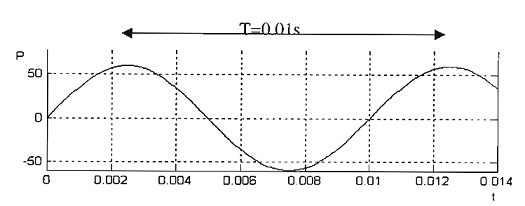
\includegraphics[scale=1]{sinwave}
    \caption{Sóng sin có biên độ 60 dB, tần số 100 Hz}
    \label{fig:c2_sinwave}
\end{figure}

Âm thanh có một số đặc trưng cơ bản như: độ cao, độ mạnh, độ dài và âm sắc.
\begin{itemize}
	\item \textbf{Độ cao} (Pitch): âm thanh luôn có một độ cao nhất định. Độ cao của âm thanh phụ thuộc vào tần số của sóng âm. Tần số càng lớn thì âm thanh càng cao, tần số càng bé thì âm thanh càng trầm.

	\begin{figure}[h]
		\centering
		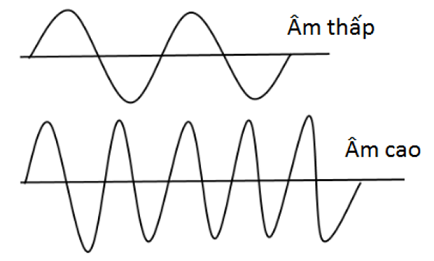
\includegraphics[scale=1]{pitch}
		\caption{Minh họa độ cao (Pitch) của âm}
		\label{fig:c2_pitch}
	\end{figure}

	\item \textbf{Độ mạnh} (Intensity): hay còn gọi là độ to của âm thanh. Độ mạnh của âm thanh phụ thuộc vào biên độ sóng âm. Biên độ càng lớn thi cường độ âm càng mạnh, biên độ càng bé thì cường độ âm càng yếu.
	\item \textbf{Độ dài} (Duration): là thời gian kéo dài của sóng âm.
	\item \textbf{Âm sắc} (Timbre): âm sắc là một đặc trưng sinh lý của âm, giúp phân biết âm thanh do các nguồn khác nhau phát ra. Âm sắc liên quan mật thiết với đồ thị giao động âm.
	\begin{figure}[h]
		\centering
		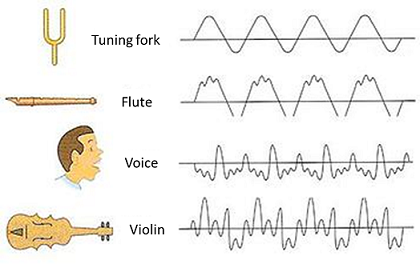
\includegraphics[scale=1]{timbre}
		\caption{Minh họa âm sắc (Timbre) của âm}
		\label{fig:c2_timbre}
	\end{figure}
\end{itemize}

\subsection{Tổng quan về tiếng nói}
Trong tự nhiên, âm thanh bao gồm nhiều loại được tạo ra từ nhiều nguồn khác nhau: 
\begin{itemize}
	\item \textbf{Âm nhạc}: âm thanh được phát ra từ các nhạc cụ.
	\item \textbf{Tiếng kêu}: được phát ra từ các loại động vật. Ví dụ: cá heo (1-164 kHz).
	\item \textbf{Tiếng động}: âm thanh phát ra từ sự va chạm giữa hai vật.
	\item \textbf{Tiếng ồn}: là những âm thanh không mong muốn.
	\item \textbf{Tiếng nói}: là những âm thanh được phát ra từ miệng con người
\end{itemize}

\noindent Ta có thể phân loại tiếng nói dựa theo thanh:
\begin{itemize}
	\item \textbf{Âm hữu thanh}: là âm khi phát ra có sự dao động của đôi dây thanh quản.
	\item \textbf{Âm vô thanh}: phát ra khi đôi dây thanh quản không dao động. Thí dụ phần cuối của phát âm English, chữ sh cho ra âm xát.
\end{itemize}

\noindent Hoặc theo âm:
\begin{itemize}
	\item \textbf{Nguyên âm}: là âm phát ra có thể kéo dài. Tất cả nguyên âm đều là âm hữu thanh, nghĩa là tuần hoàn và khá ổn định trong một đoạn thời gian vài chục ms.
	\item \textbf{Phụ âm}: là âm chỉ phát ra một nhát, không kéo dài được. Có phụ âm hữu thanh và phụ âm vô thanh.
\end{itemize}

Tiếng nói đóng vai trò quan trọng trong hoạt động động giao tiếp giữa con người, nó là phương tiện giao tiếp nhanh, tiện lợi và phổ biến nhất.

\section{Lưu trữ âm thanh trong máy tính}
Tất cả âm thanh mà chúng ta nghe được trong tự nhiên đều tồn tại dưới dạng sóng âm, là các sóng cơ học tuần hoàn liên tục analog. Trong khi đó, máy tính xử lý và lưu trữ thông tin dưới dạng các xung điện tử rời rạc digital. Vì vậy, để có thể lưu trữ và xử lý tín hiệu âm thanh trên máy tính, ta phải mô phỏng sóng âm bằng những mẫu rời rạc. Việc mô phỏng được đặc trưng bởi các thông số:
\begin{itemize}
	\item \textbf{Mẫu (Sample) là gì}: là đơn vị âm thanh nhỏ nhất được lưu trong máy tính. Để có các xung điện tử rời rạc, ta cần lấy mẫu nhiều lần từ tín hiệu analog. Mỗi mẫu là giá trị biên độ của sóng âm tại thời điểm lấy mẫu.
	\item \textbf{Tần số lấy mẫu (Sample Rate)}: là số lần lấy mẫu trên một giây, đơn vị là Hz. Tần số lấy mẫu càng cao, tín hiệu số thu được càng chính xác.
	\item \textbf{Độ dày bit (BitDepth)}: để lưu lại dưới dạng số, mỗi mẫu được biểu diễn bằng một lượng bit dữ liệu nhất định gọi là BitDepth. BitDepth càng lớn âm thanh cáng sắc nét, trung thực.
	\item \textbf{Kênh (Chanel)}: Bằng thuật toán, tín hiệu số có thể được chia thành nhiều kênh để khi nghe bằng hệ thống âm thanh vòm sẽ tạo ra cảm giác thật nhất.
\end{itemize}

Một trong những phương pháp chuyển đổi tín hiệu analog sang digital phổ biến nhất hiện nay là Pulse-Code Modulation (PCM).
Kỹ thuật PCM bao gồm 3 bước:
\begin{itemize}
	\item \textbf{Lấy mẫu (Sampling)}: quá trình rời rạc hoá tín hiệu analog đầu vào theo tần số lấy mẫu f. Ví dụ f = 44100 Hz, ta sẽ lấy mẫu 44100 lần trong một giây.
	\begin{figure}[h]
		\centering
		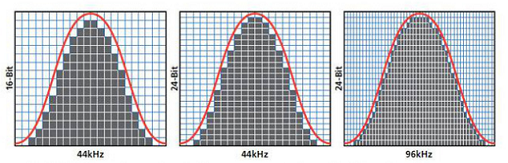
\includegraphics[scale=1]{sampling}
		\caption{Hình minh họa tín hiệu analog được lấy mẫu theo nhiều tần số khác nhau}
		\label{fig:c2_sampling}
	\end{figure}
	\item \textbf{Lượng tử hóa (Quantization)}: tín hiệu analog sau khi được lấy mẫu thì mỗi mẫu có thể có vô số các giá trị. Thay vì sử dụng giá trị mẫu chính xác, giá trị mẫu được thay bằng giá trị gần nhất trong M giá trị cho phép. Các giá trị lượng tử được gọi là các mức lượng tử, nếu các mức lượng tử cách đều nhau gọi là lượng tử đều, ngược lại gọi là lượng tử không đều. Số mức lượng tử M phụ thuộc vào số khả năng mà BitDepth có thể biểu diễn.
	\begin{figure}[h]
		\centering
		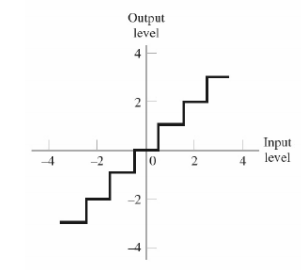
\includegraphics[scale=1]{quantization}
		\caption{Hình minh họa quá trình lượng tử hóa}
		\label{fig:c2_quantization}
	\end{figure}
	\item \textbf{Mã hóa (Encoding)}: Là quá trình biến đổi giá trị các mẫu sau khi lượng tử thành các từ mã dài n bit (n là BitDepth).
\end{itemize}

\begin{figure}[h]
    \centering
    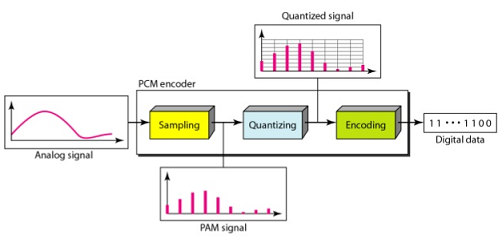
\includegraphics[scale=1]{pcm}
    \caption{Sơ đồ khối mô phỏng phương pháp PCM}
    \label{fig:c2_pcm}
\end{figure}

PCM cùng với những biến thể của nó là nền tảng cho âm thanh số. PCM sẽ sẽ hình thành một dạng sóng, sóng này ít nhiều có thể được chạy ngay bởi một bộ xử lý tín hiệu số. Trong khi hầu hết các định dạng khác khi thao tác với âm thanh thì cần thông qua các thuật toán điều khiển nên phải giải mã chúng khi sử dụng.

\subsection{Lưu trữ không nén (uncompressed)}
Các tín hiệu số thu được thông qua PCM sẽ được lưu trữ nguyên bản, không qua bất kỳ phương pháp nén hay sửa đổi.
\begin{itemize}
	\item \textbf{Ưu điểm}: khi lưu trữ dưới dạng không nén, tín hiệu âm thanh có thể được chạy ngay bởi một bộ xử lý tín hiệu số mà không cần thông qua các thuật toán giải mã.
	\item \textbf{Khuyết điểm}: kích thước tập tin âm thanh sẽ rất lớn làm hao phí không gian lưu trữ và băng thông đường truyền.
\end{itemize}
Các định dạng âm thanh tiêu biểu cho phương pháp lưu trữ không nén là: WAV, AIFF,...

\subsection{Lưu trữ nén}
Các tín hiệu số thu được thông qua PCM sẽ được nén thông qua các thuật toán khác nhau.
\begin{itemize}
	\item \textbf{Ưu điểm}: kích thước tập tin âm thanh nhỏ. Tiết kiệm không gian lưu trữ và băng thông đường truyền.
	\item \textbf{Khuyết điểm}: chất lượng âm thanh có thế bị giảm sút tùy vào thuật toán nén. Tập tin âm thanh muốn thao tác được phải thông qua quá trình giải mã
\end{itemize}

\subsubsection{Nén không mất mát (Lossless compression)}
Các tín hiệu âm thanh gốc sẽ được nén mà không mất dữ liệu và đảm bảo chất lượng ban đầu sau khi giải nén.

Để làm được điều này, cần nhờ đến nhiều thuật toán nén khác nhau. Tuy nhiên, ý tưởng chung của các thuật toán đều là tìm ra quy luật lặp của dữ liệu, sau đó tìm 1 cách hiển thị khác tối ưu hơn, tốn ít dữ liệu hơn. Ví dụ thay vì lưu chuỗi "aaaa bbb cccccc" ta sẽ chuyển thành chuỗi "a4 b3 c6" ít tốn dữ liệu hơn.

Tập tin âm thanh được nén bằng phương pháp này sẽ có tỉ lệ nén không cao, vào khoảng 1/2 đến 1/3 dung lượng âm thanh gốc.

Tiêu biểu cho phương pháp nén không mất mát là các định dạng âm thanh: FLAC, ALAC, APE,...

\subsubsection{Nén có mất mát (Lossy compression)}
Các tín hiệu âm thanh khi được nén sẽ bị loại bỏ đi các thành phần không quan trọng nhằm giảm tối đa kích thước lưu trữ. Mỗi thuật toán nén sẽ có những tiêu chí khác nhau để chọn lựa các thành phần âm thanh sẽ bị bỏ.Ví dụ, ngưỡng nghe của tai người là những âm thanh có tần số từ 14 Hz đến 20 kHz, như vậy thuật toán sẽ bỏ bớt đi các âm thanh có tần số nằm ngoài khoảng đó.

Bên cạnh đó, khi giải mã tập tin âm thanh bị nén, các thuật toán sẽ tạo ra các âm thanh giả nhằm lấp vào các phần đã bị bỏ bớt đi. Hệ quả của việc này là bạn thường nghe các âm thanh méo mó. Các tập tin nhạc được nén với tỉ lệ càng cao thì sự méo tiếng càng nhiều. Bạn sẽ rất dễ dàng nhận ra sự khác biệt khi nghe hai tập tin nhạc gốc và nhạc nén bị mất mát dữ liệu.

Tập tin âm thanh được nén bằng phương pháp này sẽ có tỉ lệ nén rất cao, lên đến 1/10 dung lượng âm thanh gốc.

Tiêu biểu cho phương pháp nén không mất mát là các định dạng âm thanh: MP3, AAC, WMA,...

\section{Ứng dụng}
Hiện nay âm thanh, tiếng nói đã được nghiên cứu và ứng dụng rộng rãi trong nhiều lĩnh vực của cuộc sống như: truyền thông, âm nhạc, chế tạo sonar,...

Trong luận văn này, tiếng nói giữ vai trò quan trọng là phương tiện tương tác chính giữa người dùng và ứng dụng. Người dùng sử dụng tiếng nói để ra lệnh cho ứng dụng, và ứng dụng sử dụng tiếng nói để phản hồi kết quả cho người dùng.

\section{Thư viện PyAudio}
\subsection{Tổng quan}
PyAudio là thư viện mã nguồn mở hỗ trợ người dùng thao tác với âm thanh trên máy tính một cách dễ dàng. PyAudio được viết bằng Python dựa trên thư viện PortAudio. PyAudio có khả năng hoạt động và cài đặt dễ dàng trên đa nền tảng: Windows, Mac OS, và Linux . Tính tới tháng 06/2017 phiên bản mới nhất của PyAudio là 0.2.11

\subsection{Chức năng}
PyAudio cũng cấp tính năng giúp người dùng dễ dàng thu và phát âm thanh từ dữ liệu thô dưới dạng từng sample. PyAudio có thể hoạt động ở chế độ đồng bộ (Synchronous) hoặc không đồng bộ (Asynchronous).

\subsection{Cài đặt}
\begin{itemize}
	\item \textbf{Windows}: python -m pip install pyaudio
	\item \textbf{Mac OS}: brew install portaudio 
pip install pyaudio
	\item \textbf{Linux}: pip install pyaudio
	\item \textbf{Build từ source}: \url{https://people.csail.mit.edu/hubert/git/pyaudio.git}
\end{itemize}

\subsection{Cách sử dụng}
\begin{lstlisting}
"""PyAudio Example: Play a wave file."""
import pyaudio
import wave
import sys
CHUNK = 1024

if len(sys.argv) < 2:
	print("Plays a wave file.\n\nUsage: %s filename.wav" % sys.argv[0])
	sys.exit(-1)

wf = wave.open(sys.argv[1], 'rb')
# instantiate PyAudio (1)
p = pyaudio.PyAudio()
# open stream (2)
stream = p.open(format=p.get_format_from_width(wf.getsampwidth()),
                channels=wf.getnchannels(),
                rate=wf.getframerate(),
                output=True)
# read data
data = wf.readframes(CHUNK)

# play stream (3)
while len(data) > 0:
	stream.write(data)
	data = wf.readframes(CHUNK)

# stop stream (4)
stream.stop_stream()
stream.close()
# close PyAudio (5)
p.terminate()
\end{lstlisting}

Đoạn code trên minh họa cách sử dụng thư viện PyAudio để phát âm thanh từ một file WAV. Chúng tôi sẽ dùng nó để hướng dẫn cách sử dụng đơn giản thư viện PyAudio
\begin{itemize}
	\item Để sử dụng thư viện PyAudio, trước hết cần khởi tạo PyAudio bằng cách sử dụng câu lệnh textbf{pyaudio.PyAudio()} (1). Câu  lệnh này sẽ khởi tạo thư viện PortAudio bên dưới.
	\item Để có thể thu âm hoặc phát audio, ta mở các stream tương ứng bằng câu lệnh \textbf{pyaudio.PyAudio.open()} (2). Input stream để thu âm, output stream để phát audio. Một số tham số cần chú ý trong câu lệnh này:
	\begin{itemize}
		\item \textbf{format}: là định dạng được sử dụng khi encoding. Định dạng này phụ thuộc vào số lượng bit dùng để mã hóa một mẫu (BitDepth).
		\item \textbf{chanels}: số lượng kênh của tập tin âm thanh cần phát hoặc số lượng kênh của âm thanh cần thu âm.
		\item \textbf{rate}: là tần số lấy mẫu (Sample Rate)
		\item \textbf{output}: giá trị này bằng \textbf{true} thì đây là stream output dùng để phát âm thanh.
		\item \textbf{input}: giá trị này bằng \textbf{true} thì đây là stream input dùng để thu âm thanh.
	\end{itemize}
	\item Khi cần phát âm thanh, ta ghi dữ liệu âm thanh lên output stream bằng hàm \textbf{pyaudio.Stream.write()}. Khi cần thu âm thanh, ta đọc dữ liệu âm thanh thu được từ input stream thông qua hàm \textbf{pyaudio.Stream.read()} (3). Đoạn code minh họa đang chạy ở chế độ blocking, nên các hàm \textbf{pyaudio.Stream.write()} và \textbf{pyaudio.Stream.read()} sẽ block chương trình đến khi chúng thực hiện việc đọc/ghi xong.
	\item Để tạm dừng đọc/ghi âm thanh ta dùng hàm \textbf{pyaudio.Stream.stop\_stream()}. Để kết thúc stream ta dùng hàm \textbf{pyaudio.Stream.close()} (4).
	\item Cuối cùng để giải phóng PortAudio ta dùng hàm \textbf{pyaudio.PyAudio.terminate()} (5).
\end{itemize}

\subsection{Các ưu, khuyết điểm}
\begin{itemize}
	\item \textbf{Ưu điểm}: thư viện cài đặt đơn giản, hỗ trợ chạy trên nhiều hệ điều hành.
	\item \textbf{Nhược điểm}: thư viện hỗ trợ ít tính năng. Không hỗ trợ thu âm đồng thời từ nhiều micro.
\end{itemize}

\subsection{Ứng dụng}
Trong luận văn này, thư viên PyAudio đảm nhận vai trò thu âm giọng nói của người dùng. Cung cấp thông tin cho các thành phần khác của hệ thống xử lý.






\chapter{Speech to Text}
\ifpdf
    \graphicspath{{Chapter3/Chapter3Figs/PNG/}{Chapter3/Chapter3Figs/PDF/}{Chapter3/Chapter3Figs/}}
\else
    \graphicspath{{Chapter3/Chapter3Figs/EPS/}{Chapter3/Chapter3Figs/}}
\fi

\textit{Nội dung chương 3 sẽ giới thiệu tổng quan về bài toán Speech to Text, mô hình hoạt động, các ứng dụng của Speech to Text, các vấn đề cần giải quyết của module Speech to Text trong một hệ thống trợ lý ảo và cách giải quyết các vấn đề đó. Chương 3 cũng sẽ giới thiệu về chức năng, cách cài đặt, cách sử dụng cũng như các ưu nhược điểm của các thư viện pocketsphinx và Google Speech to Text.}

\section{Tổng quan}

Speech to Text, hay Speech Recognition là một lĩnh vực trong khoa học máy tính, trong đó nghiên cứu và phát triển các phương pháp và công nghệ để máy tính có thể nhận biết và chuyển đổi ngôn ngữ nói sang dạng văn bản. Speech recognition là một bài toán khó dành cho các nhà khoa học, vì tiếng nói luôn thay đổi theo thời gian và có sự khác biệt giữa tiếng nói của những người khác nhau, tốc độ nói, ngữ cảnh và môi trường khác nhau.

Những hệ thống speech recognition đầu tiên trên thế giới có khả năng nhận biết rất hạn chế: số lượng từ vựng mà chúng có thể nhận biết chỉ ở mức vài chục, và chỉ có thể nhận biết chính xác nếu người dùng nói một cách rất rõ ràng. Ngày nay, với sự phát triển bùng nổ của deep learning và big data, các công nghệ speech recognition cũng đã phát triển rất nhanh về số lượng từ vựng và độ chính xác. Các hệ thống speech recognition hiện đại nhất có thể nhận biết được hàng chục nghìn, thậm chí là hàng trăm nghìn từ khác nhau, và độ lỗi khi nhận biết đã giảm đến gần mức nhận biết của con người. Ngày càng nhiều công ty công nghệ đã tham gia vào cuộc đua về speech recognition, có thể kể đến Google, Microsoft, IBM, Baidu, Apple, Amazon,...

\section{Mô hình hoạt động}

Hiện nay có rất nhiều kỹ thuật khác nhau để phát triển speech recognition. Tuy nhiên có thể nhận thấy một điểm chung của đa phần các kỹ thuật này là các mô hình thống kê, trong đó nổi bật là Hidden Markov Model (HMM).

Khi huấn luyện, các câu nói trong tập dữ liệu sẽ thường được chia thành các thành phần âm (phonemes), tín hiệu âm thanh đầu vào thường sẽ được chia thành những đoạn ngắn, đưa qua các bước tiền xử lý như FFT hoặc MFCC để trích xuất đặc trưng. Hệ thống speech recognition sẽ sử dụng HMM để tìm sự liên hệ giữa các phonemes và các đặc trưng của tín hiệu âm thanh. Khi đó, khi một đoạn âm thanh mới được đưa vào, HMM sẽ trả về những chuỗi âm có thể tương ứng với đoạn âm thanh đó. Mô hình này được gọi là acoustic model.

Bên cạnh acoustic model, người ta cũng sẽ tạo ra các language model. Language model thường sẽ gồm:

\begin{itemize}
    \item Danh sách các từ (gọi là từ điển). Hệ thống sẽ nhận biết được những từ nằm trong từ điển này.
    \item Cấu trúc âm của các từ trong từ điển, ví dụ như từ "stuff" gồm 3 âm: "st", "uh" và "ff".
    \item Mối quan hệ giữa các từ trong từ điển (từ nào thường đứng cạnh từ nào).
\end{itemize}

Language model sẽ nhận các chuỗi âm output từ acoustic model, tìm cách ghép các chuỗi âm này thành các chuỗi từ có trong từ điển, và tìm cách ghép các chuỗi từ này thành câu.

\begin{figure}[h]
    \centering
    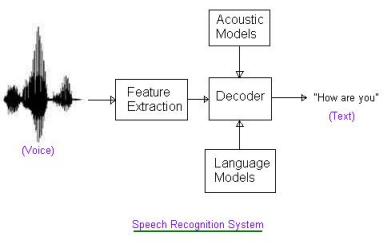
\includegraphics[scale=1]{SRSystem}\footnotemark
    \caption{Cấu trúc một hệ thống speech recognition đơn giản}
    \label{fig:c3_SRSystem}
\end{figure}

\footnotetext{http://www.rfwireless-world.com/Terminology/automatic-speech-recognition-system.html}

Ngoài HMM, nhiều mô hình khác cũng đã được các nhà phát triền speech recognition sử dụng để thay thế hoặc hỗ trợ cho HMM như Gaussian Mixture Model, Deep Neural Networks, Recurrent Neural Networks, Finite-State Transducers...

\section{Ứng dụng}

\begin{itemize}
    \item Chuyển hướng cuộc gọi tự động, quay số bằng giọng nói, tìm kiếm bằng giọng nói.
    \item Dùng trong việc ra lệnh bằng giọng nói trên các máy bay quân sự.
    \item Dùng trong các ứng dụng dạy học ngoại ngữ.
    \item Phụ đề tự động trong các video.
    \item Điều khiển robot bằng giọng nói.
    \item Hỗ trợ người khuyết tật.
    \item Phiên dịch tự động.
    \item ...
\end{itemize}

\section{Các vấn đề cần giải quyết}

Speech to Text luôn đóng vai trò là một trong những phần quan trọng nhất trong một ứng dụng trợ lý ảo. Trong một hệ thống trợ lý ảo điển hình, sẽ có hai vấn đề lớn về speech recognition: dò tìm keyword và chuyển đổi lệnh của người dùng thành văn bản.

\subsection{Dò tìm keyword}

Mỗi hệ thống trợ lý ảo sẽ được xác định trước một keyword, keyword này sẽ được dùng để kích hoạt trợ lý ảo. Mỗi khi người dùng gọi keyword này, ứng dụng sẽ chuyển sang trạng thái thu âm để ghi nhận lệnh từ phía người dùng. Keyword này thường là một từ hoặc cụm từ ngắn, dễ phát âm và dễ nhận biết, và thường chứa tên của ứng dụng, ví dụ như của Google Assistant là "OK Google", của Siri là "Hey Siri",...

\subsubsection{Yêu cầu}

Thứ nhất, chức năng dò tìm keyword của hệ thống phải hoạt động liên tục trong suốt quá trình ứng dụng chạy, do hệ thống phải có phản ứng ngay lập tức khi người dùng gọi keyword. Nếu chức năng này bị gián đoạn, hệ thống sẽ dễ bỏ lỡ mất keyword. Do đó, phần nhận biết tiếng nói trong chức năng này nên hoạt động offline, để tránh những gián đoạn trên đường mạng.

Thứ hai, tốc độ nhận biết keyword phải rất nhanh. Hệ thống sẽ liên tục thu âm từ microphone thành các frame âm thanh để xử lý liên tục trong thời gian thực, và phải liên tục kiểm tra các đoạn âm thanh liên tiếp nhau xem có chứa keyword hay không. Khi phát hiện ra một đoạn âm thanh thu được có chứa keyword, hệ thống phải ngay lập tức phản hồi lại cho người dùng và chuyển sang trạng thái thu âm lệnh của người dùng. Nếu tốc độ nhận biết keyword chậm, việc chuyển trạng thái sang thu âm sẽ bị trễ, và lệnh của người dùng khi thu vào có thể sẽ không đầy đủ, dẫn tới phản hồi sai.

Thứ ba, độ chính xác của việc nhận biết keyword phải đạt mức tương đối cao. Do từ khóa được chọn là một từ dễ đọc và dễ nhận biết nên độ chính xác của chức năng này không cần phải quá cao. Ngoài ra việc đặt ngưỡng nhận biết ở mức không quá cao sẽ làm hạn chế tối đa số lượng false negatives (trường hợp người dùng gọi keyword nhưng ứng dụng không nhận ra). Tuy nhiên điều đó sẽ làm gia tăng số lượng false positives (trường hợp người dùng không gọi keyword nhưng ứng dụng lại nhận ra), do đó cần phải tìm giải pháp để giảm số lượng false positives này.

\subsubsection{Giải pháp}

Trong hệ thống này, chúng tôi sẽ sử dụng thư viện pocketsphinx để cài đặt chức năng phát hiện keyword. Đây là một thư viện speech recognition có khả năng hoạt động offline, tốc độ xử lý nhanh, tuy nhiên độ lỗi của thư viện này là lớn hơn so với một vài thư viện khác.

Ngoài ra, ngay khi pocketsphinx nhận ra được keyword trong một đoạn âm thanh, hệ thống sẽ gửi đoạn âm thanh đó vào thư viện Google Speech to Text để kiểm tra lại một lần nữa. Hai bước kiểm tra qua hai model khác nhau sẽ giúp hệ thống hạn chế được số lượng false positives.

\subsection{Chuyển đổi lệnh người dùng thành văn bản}

Sau khi phát hiện ra keyword, hệ thống sẽ được kích hoạt và bắt đầu thu âm lệnh của người dùng. Sau khi người dùng nói xong, hệ thống sẽ phải chuyển lệnh của người dùng sang dạng văn bản để có thể xử lý và hiểu được lệnh đó.

\subsubsection{Yêu cầu}

Phần chức năng chuyển đổi câu lệnh của người dùng thành văn bản chỉ bắt đầu hoạt động khi người dùng muốn ra lệnh, tức là sau khi người dùng gọi keyword, còn những khoảng thời gian khác, chức năng này sẽ nằm ở trạng thái chờ. Việc thu âm lệnh người dùng chỉ ngừng lại khi người dùng ngừng ra lệnh. Nếu hệ thống ngừng thu âm quá sớm, lệnh của người dùng thu vào sẽ bị thiếu và không chính xác. Nếu hệ thống ngừng thu âm quá muộn sẽ tạo ra độ trễ lớn từ lúc người dùng ra lệnh đến lúc ứng dụng phản hồi, và có thể tạp âm sau khi người dùng nói xong sẽ lọt vào phần speech recognition khiến kết quả nhận biết bị sai lệch.

Ngoài ra, độ chính xác của việc chuyển lệnh của người dùng về văn bản phải đạt mức rất cao, để đảm bảo hệ thống có thể hiểu đúng được ý định của người dùng.

\subsubsection{Giải pháp}

Trong hệ thống trợ lý ảo này, module chuyển đổi lệnh người dùng thành văn bản được cài đặt sử dụng thư viện Google Speech to Text. Đây là công cụ nhận biết tiếng nói của Google được đánh giá rất cao về độ chính xác, nhờ đó hệ thống sẽ đảm bảo hiểu đúng được hầu hết các lệnh của người dùng.

Để việc thu âm có thể ngừng đúng lúc, trong hệ thống sẽ có một giá trị thời gian $T$ và một ngưỡng cường độ $D$. Khi âm thanh thu được từ microphone có cường độ nằm dưới mức $D$ trong một khoảng thời gian $T$ liên tục thì hệ thống sẽ xem như người dùng đã kết thúc việc ra lệnh và dừng trạng thái thu âm để bắt đầu xử lý đoạn âm thanh đã thu được.

\section{Thư viện pocketsphinx}

\subsection{Tổng quan}

Pocketsphinx là một thư viện speech recognition mã nguồn mở được phát triển bởi Viện Công nghệ Ngôn Ngữ, thuộc trường Đại học Carnegie Mellon (Mỹ). Pocketsphinx là phiên bản tối ưu của CMU Sphinx-II, cũng là một hệ thống nhận dạng tiếng nói khá nổi tiếng của ĐH Carnegie Mellon. Nhóm nghiên cứu này đã tối ưu hóa pocketsphinx rất nhiều về bộ nhớ và thuật toán, nhằm có thể tạo ra một thư viện nhận dạng tiếng nói liên tục có khả năng đưa vào các thiết bị cầm tay.

Hệ thống của pocketsphinx chủ yếu dựa trên những mô hình phổ biến của speech recognition như Gaussian Mixture Model và thuật toán Viterbi trên Hidden Markov Model, kết hợp với nhiều thuật toán hỗ trợ khác\cite{huggins2006pocketsphinx}.

Pocketsphinx được đánh giá cao nhờ vào khả năng hoạt động offline và tốc độ xử lý khá nhanh. Ngoài ra, pocketsphinx có khả năng xử lý real-time liên tục trên stream âm thanh (thay vì phải hoàn tất việc thu âm và xử lý trên file âm thanh thu được).

\subsection{Cách cài đặt}

\subsection{Cách sử dụng}

các thông số của thư viện

\subsection{Các ưu, nhược điểm}

\begin{itemize}
    \item \textbf{Ưu điểm:} Hỗ trợ xử lý offline, xử lý real-time liên tục, hỗ trợ chức năng dò tìm keyword.
    \item \textbf{Nhược điểm:} Độ chính xác khá kém. Độ lỗi word error rate khi thử nghiệm của pocketsphinx lên đến 13.95\%\cite{huggins2006pocketsphinx}.
\end{itemize}

\subsection{Ứng dụng}

Trong hệ thống trợ lý ảo của khóa luận này, pocketsphinx sẽ được sử dụng trong module WakeUp. Pocketsphinx sẽ giúp phát hiện ra khi người dùng gọi wake-up word, qua đó kích hoạt hệ thống.

\section{Thư viện Google Speech To Text}

\subsection{Tổng quan}

Google Speech Recognition là hệ thống nhận biết tiếng nói do Google nghiên cứu và phát triển. Hệ thống này đã được Google tích hợp vào trợ lý ảo Google Assistant trên các thiết bị Android và loa thông minh Google Home, và cũng đã được đưa vào ứng dụng tìm kiếm Google Search. Google cũng đã đưa ra Google Speech API cho phép các lập trình viên sử dụng hệ thống speech recognition này vào các ứng dụng của họ. Google Speech to Text là một thư viện trên Python có khả năng nhận biết tiếng nói nhờ vào việc gọi đến Google Speech API.

Trong quá trình phát triển, các nhà nghiên cứu của Google đã sử dụng nhiều kỹ thuật khác nhau cho Google Speech Recognition, từ những kỹ thuật cổ điển như Gaussian Mixture Model, đến những kỹ thuật hiện đại hơn như Deep Neural Networks hay Long Short-term Memory Recurrent Neural Networks (LSTM RNNs)\cite{beaufays}.

Nhờ sự thay đổi và tiến bộ liên tục, Google Speech Recognition được đánh giá rất cao về độ chính xác của mình. Tại Google I/O 2017, Google đã công bố độ chính xác của công nghệ nhận biết tiếng nói này đã đạt độ lỗi word error rate là 4.9\%\cite{protalinski}, tức là độ chính xác lên đến hơn 95\%.

\subsection{Cách cài đặt}

\subsection{Cách sử dụng}

Các thông số của thư viện

\subsection{Các ưu, nhược điểm}

\begin{itemize}
    \item \textbf{Ưu điểm:} Độ chính xác rất cao.
    \item \textbf{Nhược điểm:} Yêu cầu internet để hoạt động, không xử lý real-time trên stream âm thanh được mà phải gửi toàn bộ file âm thanh.
\end{itemize}

\subsection{Ứng dụng}

Trong hệ thống này, thư viện Google Speech to Text được dùng trong module SpeechToText. Module này sẽ đóng vai trò chuyển đổi những câu lệnh của người dùng từ dạng âm thanh sang dạng văn bản.

\chapter{Text To Speech}
\ifpdf
    \graphicspath{{Chapter4/Chapter4Figs/PNG/}{Chapter4/Chapter4Figs/PDF/}{Chapter4/Chapter4Figs/}}
\else
    \graphicspath{{Chapter4/Chapter4Figs/EPS/}{Chapter4/Chapter4Figs/}}
\fi
\textit{Nội dung chương 4 sẽ giới thiệu tổng quan về bài toán Text to Speech, mô hình hoạt động, các ứng dụng của Text to Speech, các vấn đề cần giải quyết của module Text to Speech trong một hệ thống trợ lý ảo và cách giải quyết các vấn đề đó. Chương 4 cũng sẽ giới thiệu về chức năng, cách cài đặt, cách sử dụng cũng như các ưu nhược điểm của các thư viện iSpeech và Google Text to Speech.}

\section{Tổng quan}
Text to Speech (TTS), hay còn gọi là hệ thống tổng hợp giọng nói,  là một lĩnh vực trong khoa học máy tính. Text to Speech nghiên cứu phương pháp tạo ra giọng nói nhân tạo từ văn bản. Giọng nói nhân tạo này được đánh giá dựa trên hai tiêu chí: mức độ tự nhiên và mức độ dễ nghe. Mức độ tự nhiên chỉ sự tương đồng về ngữ điệu của giọng nói tổng hợp với giọng nói con người. Mức độ dễ nghe đánh giá khả năng phát âm rõ ràng, và khả năng nghe hiểu của con người với giọng nói tổng hợp. Việc có quá nhiều ngôn ngữ trên thế giới, cộng thêm việc mỗi ngôn ngữ lại có nhiều ngữ điệu khác nhau tùy vùng miền đã đặt ra những thách thức không hề đơn giản cho các nhà khoa học.

Text to Speech đã được bắt đầu phát triển từ rất lâu trước đây và đã trải qua một quá trình cải tiến lâu dài. Có thể nói khởi nguồn của nó là mô hình bắt chước giọng nói người với năm nguyên âm (u, e, o , a, i), được phát triển vào năm 1779 bởi nhà khoa học người Đan Mạch Christian Kratzenstein tại viện hàn lâm khoa học Nga. Từ đó đến nay, sau nhiều năm phát triển cải tiến, hệ thống tổng hợp giọng nói đã có nhiều bước phát triển vượt bật, giọng nói tạo ra ngày càng giống với ngữ điệu người và hỗ trợ nhiều loại ngôn ngữ trên thế giới. Hiện nay, có rất nhiều công ty tham gia vào phát triển hệ thống Text to Speech, trong đó nổi bật là các công ty: Google, Microsoft, iSpeech, Amazon,...

\section{Mô hình hoạt động}
Một hệ thống Text to Speech thông thường bao gồm hai thành phần chính: front-end và back-end.
\begin{itemize}
\item Front-end, hay bộ phận tiền xử lý (Pre-processor), thực hiện ba nhiệm vụ chính. 
	\begin{itemize}
		\item Phân đoạn (Tokenization): là quá trình phân tích cấu trúc của đoạn văn. Quá trình này phân phia và đánh dấu văn bản thành từng từ, nhóm từ, mệnh đề, câu văn và đoạn văn.
		\item Chuẩn hóa (Normalization): là quá trình chuyển đổi các ký tự số, ký tự đặc biệt, viết tắt trong văn bản về dạng viết đầy đủ. Ví dụ "Dr"  sẽ được chuyển đổi thành "doctor". 
		\item Phân tích ngôn ngữ (Linguistic analysis): bao gồm phân tích hình thái học (Morphological analysis) để tìm ra cách phát âm tương ứng của từng từ và phân tích cú pháp (Syntactic analysis) nhằm hiểu cách diễn đạt hay nhấn mạnh của từ.
	\end{itemize}
\item Back-end, còn gọi là bộ phận tổng hợp âm thanh (Speech synthesizer). Nhiệm vụ của phần này là tổng hợp các thông tin từ front-end thành giọng nói ở dạng sóng âm thanh.
\end{itemize}
\begin{figure}[h]
    \centering
    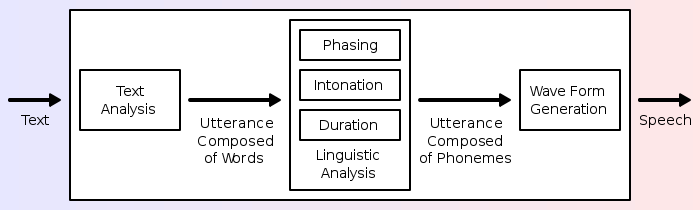
\includegraphics[scale=1]{ttsmodel}
    \caption{Minh họa mô hình hoạt động của hệ thống Text to Speech}
    \label{fig:c4_ttsmodel}
\end{figure}

\indent Có nhiều kỹ thuật dùng trong tổng hợp âm thanh. Tùy thuộc vào đặc tả của hệ thống, thiên về mức độ dễ nghe, thiên về mức độ tự nhiên, hay đồng thời cả hai tính chất trên mà sẽ lựa chọn kỹ thuật thích hợp. Có hai kỹ thuật chính thường được dùng là tổng hợp ghép nối và tổng hợp cộng hưởng tần số, ngoài ra còn có một số kỹ thuật khác.
\begin{itemize}
\item \textbf{Tổng hợp ghép nối}: Tổng hợp ghép nối dựa trên việc nối vào nhau các đoạn âm thanh của một giọng nói đã được ghi âm. Thông thường, tổng hợp ghép nối tạo ra giọng nói tương đối tự nhiên. Tuy nhiên, giọng nói tự nhiên được ghi âm có sự thay đổi từ lần phát âm này sang lần phát âm khác, và công nghệ tự động hóa việc ghép nối các đoạn của sóng âm thỉnh thoảng tạo ra những tiếng cọ xát không tự nhiên ở phần ghép nối. Có ba kiểu tổng hợp ghép nối.
\begin{itemize}
\item \textbf{Tổng hợp chọn đơn vị}: Tổng hợp chọn đơn vị dùng một cơ sở dữ liệu lớn các giọng nói ghi âm (thông thường dài hơn 1 giờ đồng hồ ghi âm). Trong lúc ghi âm, mỗi câu phát biểu được tách ra thành các đơn vị khác như: các âm tỏ lời đơn lẻ, âm tiết, hình vị, từ, nhóm từ, và câu văn. Thông thường, việc tách ra như vậy cần một máy nhận dạng tiếng nói được đặt ở chế độ khớp với văn bản viết tương ứng với đoạn ghi âm, và dùng đến hiển thị sóng âm và phổ âm thanh. Một bảng tra các đơn vị được lập ra dựa trên các phần đã tách và các thông số âm học như tần số cơ bản, thời lượng, vị trí của âm tiết, và âm tỏ lời gần đó. Khi chạy, các câu phát biểu được tạo ra bằng cách xác định chuỗi đơn vị phù hợp nhất từ cơ sở dữ liệu. Quá trình này được gọi là chọn đơn vị, và thường cần dùng đến cây quyết định để thực hiện.

Kỹ thuật chọn đơn vị tạo ra độ tự nhiên cao do không áp dụng các kỹ thuật xử lý tín hiệu số lên các đoạn giọng nói đã ghi âm, tuy rằng một số hệ thống có thể áp dụng xử lý tín hiệu tại các đoạn nối giữa các đơn vị để làm liền mạch kết quả sau khi ghép nối. Thực tế, các hệ thống chọn đơn vị có thể tạo ra giọng nói không thể phân biệt được với người thật. Tuy nhiên, để đạt độ tự nhiên cao, thường cần một cơ sở dữ liệu lớn chứa các đơn vị để lựa chọn; có thể lên tới vài gigabyte, tương đương với hàng chục giờ ghi âm.

\item \textbf{Tổng hợp âm kép}: Tổng hợp âm kép dùng một cơ sở dữ liệu giọng nói nhỏ chứa tất cả các âm kép (chuyển tiếp âm thanh) xuất hiện trong ngôn ngữ đang xét. Số lượng âm kép phụ thuộc vào đặc tính ghép âm học của ngôn ngữ: tiếng Tây Ban Nha có 800 âm kép, tiếng Đức có 2500. Trong tổng hợp âm kép, chỉ có một ví dụ của âm kép được chứa trong cơ sở dữ liệu. Khi chạy, lời văn được chồng lên các đơn vị này bằng kỹ thuật xử lý tín hiệu số như mã tiên đoán tuyến tính, PSOLA hay MBROLA.

Chất lượng của âm thanh tổng hợp theo cách này thường không cao bằng phương pháp chọn đơn vị nhưng tự nhiên hơn tổng hợp cộng hưởng tần số. Tổng hợp âm kép tạo ra các tiếng cọ xát ở phần ghép nối và đôi khi giọng nói kiểu robot do các kỹ thuật xử lý tín hiệu số gây ra. Lợi thế của phương pháp này là kích thước cơ sở dữ liệu nhỏ. Các ứng dụng thương mại của phương pháp này đang ít dần, tuy nhiên có nhiều hệ thống như thế này được phân phát tự do, và phục vụ cho nghiên cứu.

\item \textbf{Tổng hợp chuyên ngành}: Tổng hợp chuyên biệt ghép nối các từ và đoạn văn đã được ghi âm để tạo ra lời phát biểu. Nó được dùng trong các ứng dụng có các văn bản chuyên biệt cho một chuyên ngành, sử dụng lượng từ vựng hạn chế, như các thông báo chuyến bay hay dự báo thời tiết.

Công nghệ này rất đơn giản, và đã được thương mại hóa từ lâu, đã đi vào các đồ vật như đồng hồ biết nói hay máy tính bỏ túi biết nói. Mức độ tự nhiên của các hệ thống này có thể rất cao vì số lượng các câu nói không nhiều và khớp với lời văn và âm điệu của giọng nói ghi âm. Tuy nhiên các hệ thống này bị hạn chế bởi cơ sở dữ liệu chuyên ngành, không phục vụ mọi mục đích mà chỉ hoạt động với các câu nói mà chúng đã được lập trình sẵn.
\end{itemize}

\item \textbf{Tổng hợp cộng hưởng tần số}: Tổng hợp cộng hưởng tần số không sử dụng bất cứ mẫu giọng thật nào khi chạy. Thay vào đó, tín hiệu âm thanh cho ra dựa trên một mô hình âm thanh. Các thông số như tần số cơ bản, sự phát âm, và mức độ tiếng ồn được thay đổi theo thời gian để tạo ra dạng sóng cho giọng nói nhân tạo. Phương pháp này đôi khi còn được gọi là tổng hợp dựa trên quy tắc, dù cho nhiều hệ thống ghép nối mẫu âm thanh thật cũng có dùng các thành phần dựa trên quy tắc.

Nhiều hệ thống dựa trên tổng hợp cộng hưởng tần số tạo ra giọng nói nhân tạo, như giọng rôbốt, không tự nhiên, và phân biệt rõ ràng với giọng người thật. Tuy nhiên độ tự nhiên cao không phải lúc nào cũng là mục đích của hệ thống và hệ thống này cũng có các ưu điểm riêng của nó.

Hệ thống này nói khá dễ nghe, ngay cả ở tốc độ cao, không có tiếng cọ xát do ghép âm tạo ra. các hệ thống này hoạt động ở tốc độ cao, có thể hướng dẫn người khiếm thị nhanh chóng dò dẫm trên máy tính, bằng cách đọc to những gì hiện ra trên màn hình. Các hệ thống này cũng nhỏ gọn hơn các hệ thống ghép nối âm, vì không phải chứa cơ sở dữ liệu mẫu âm thanh lớn. Nó có thể dùng trong các hệ thống nhúng khi bộ nhớ và tốc độ xử lý có hạn. Hệ thống này cũng có khả năng điều khiển mọi khía cạnh của tín hiệu âm thanh đi ra, no cho ra một dải rộng các lời văn và ngữ điệu, và không chỉ thể hiện được câu nói thường hay câu hỏi, mà cả các trạng thái tình cảm thông qua âm điệu của giọng nói.

Các ví dụ về các hệ thống cho ra ngữ điệu chính xác (nhưng không cho ra ngay lập tức sau khi nhận đầu vào) là các công trình cuối những năm 1970 của đồ chơi Speak \& Spell của Texas Instruments, và các trò chơi video của SEGA đầu những năm 1980 như: Astro Blaster, Zektor, Space Fury, và Star Trek. Hiện vẫn chưa có hệ thống cho ra intonation chính xác ngay sau khi nhận văn bản đầu vào.

\item \textbf{Tổng hợp mô phỏng phát âm}: Tổng hợp mô phỏng phát âm là các kỹ thuật tổng hợp giọng nói dựa trên mô hình máy tính của cơ quan phát âm của người và quá trình phát âm xảy ra tại đó. Hệ thống tổng hợp mô phỏng phát âm đầu tiên là ASY, thường được dùng cho các thí nghiệm trong nghiên cứu, được phát triển ở phòng thí nghiệm Haskins vào giữa những năm 1970 bởi Philip Rubin, Tom Baer, và Paul Mermelstein. ASY dựa trên mô hình cơ quan phát âm đã được tạo ra bởi phòng thí nghiệm Bell vào những năm 1960 và 1970 bởi Paul Mermelstein, Cecil Coker, và các đồng nghiệp khác. Tổng hợp mô phỏng phát âm đã từng chỉ là hệ thống dành cho nghiên cứu khoa học cho mãi đến những năm gần đây. Lý do là rất ít mô hình tạo ra âm thanh chất lượng đủ cao hoặc có thể chạy hiệu quả trên các ứng dụng thương mại. Một ngoại lệ là hệ thống dựa trên NeXT; vốn được phát triển và thương mại hóa bởi Trillium Sound Research Inc, ở Calgary, Alberta, Canada. Đây là một công ty tách ra từ Đại học Calgary nơi các nghiên cứu ban đầu đã được thực hiện. Theo sau các vụ chuyển nhượng các từng phần của NeXT (bắt đầu từ Steve Jobs vào cuối những năm 1980 và việc hợp nhất với Apple năm 1997), phần mềm của Trillium được phân phát với giấy phéo tự do GPL. Dự án gnuspeech, một dự án của GNU, tiếp tục phát triển phần mềm này. Phần mềm gốc NeXT và các chuyển đổi sang cho Mac OS/X và GNUstep trong GNU/Linux có thể tìm thấy tại trang GNU savannah; chúng đều kèm theo tài liệu hướng dẫn trực tuyến và các bài viết liên quan đến lý thuyết nền tảng của công trình. Hệ thống, vốn được thương mại hóa lần đầu vào năm 1994, tạo ra một máy tổng hợp giọng nói dựa trên mô phỏng phát âm hoàn chỉnh, dựa trên mô hình ống dẫn sóng tương đương với cơ quan phát âm của người. Nó được điều khiển bởi Mô hình Phần Riêng biệt của Carré; bản thân mô hình này lại dựa trên công trình của Gunnar Fant và các người khác ở Phòng thí nghiệm Công nghệ Giọng nói Stockholm thuộc Viện Cộng nghệ Hoàng gia Thụy Điển về tổng hợp giọng nói cộng hưởng tần số. Công trình này cho thấy các cộng hưởng tần số trong ống cộng hưởng có thể được điều khiển bằng cách thay đổi tám tham số tương đồng với các cách phát âm tự nhiên của cơ quan phát âm của người. Hệ thống bao gồm một từ điển phát âm cùng với các quy tắc phát âm tùy thuộc ngữ cảnh để giúp ghép nối âm điệu và tạo ra các tham số phát âm; mô phỏng theo nhịp điệu và ngữ điệu thu được từ các kết quả nghiên cứu ngữ âm học.

\item \textbf{Tổng hợp lai}: Các hệ thống tổng hợp lai kết hợp các yếu tố của tổng hợp cộng hưởng tần số với tổng hợp ghép nối để giảm thiểu các tiếng cọ xát khi ghép nối các đoạn âm thanh.

Một ví dụ là RecSimCat, phát triển bởi Shakti Singh Parmar có thể tạo ra giọng dễ nghe và tự nhiên.[cần dẫn nguồn]

\item \textbf{Tổng hợp dựa trên HMM}
Tổng hợp dựa trên HMM là một phương pháp dựa vào mô hình Markov ẩn (HMM, viết tắt cho thuật ngữ tiếng Anh Hidden Markov model). Trong hệ thống này, phổ tần số của giọng nói, tần số cơ bản, và thời lượng đều được mô phỏng cùng lúc bởi HMM. Dạng sóng của giọng nói được tạo từ mô hình Markov ẩn dựa trên tiêu chí khả thực cực đại.
\end{itemize}

\section{Ứng dụng}
Hệ thống Text to Speech đang được nghiên cứu và ứng dụng trong nhiều lĩnh vực:
\begin{itemize}
	\item Máy đọc văn bản dùng cho những người mù chũ, có thị lực kém hoặc khiếm thị.
	\item Dùng trong ngành công nghiệp robot.
	\item Là công cụ giao tiếp của các trợ lý ảo.
	\item Trong luận văn này, hệ thống Text to Speech được sử dụng làm phương tiện để ứng dụng phản hồi lại lệnh của người dùng.
\end{itemize}

\section{Thư viện Google Text To Speech (gTTS)}
\subsection{Tổng quan}
gTTS là thư viện mã nguồn mở, được viết bằng ngôn ngữ python và hỗ trợ hoạt động trên đa nền tảng. Thư viện này được phát triển bởi Pierre Nick Durette một lập trình viên người Canada.
gTTS là một thư viện bao phủ trên nền Google's Text to Speech API cung cấp các tính năng giúp người dùng tương tác đơn giản hơn với hệ thống Text to Speech API của Google.

\subsection{Chức năng}
Thư viện gTTS có chứ năng chuyển một đoạn văn bản thanh giọng nói dưới dạng tập tin mp3. Thư viện này không giới hạn số từ của văn bản bằng cách chia đoạn văn bản ra thành các câu ngắn hơn tại các vị trí mà khi nói giọng người sẽ tạm ngừng một cách tự nhiên.

\subsection{Cách cài đặt}
\begin{itemize}
\item Windows, Mac OS, Linux: pip install gTTS
\end{itemize}

\subsection{Cách sử dụng}
Thư viện gTTS có thể được sử dụng như là một python module hoặc chạy trên command line
You may either use gTTS as a python module or as a command-line utility
\begin{itemize}
\item Python Module
\begin{lstlisting}
# Import gTTS
from gtts import gTTS

# Create an instance
 tts = gTTS(text='Hello', lang='en', slow=True)
#Parameters:
#text - String - Text to be spoken.
#lang - String - ISO 639-1 language code (supported by the Google Text to Speech API) to speak in.
#slow - Boolean - Speak slowly. Default False (Note: only two speeds are provided by the API).

#Write to a file
#To disk using save(file_name)
tts.save("hello.mp3")

#To a file pointer using write_to_fp(file_object)
f = TemporaryFile()
tts.write_to_fp(f)
# <Do something with f>
f.close()
\end{lstlisting}
\item Command line
\begin{lstlisting}
gtts-cli.py [-h] (["text to speak"] | -f FILE) [-l LANG] [--slow] [--debug] [-o destination_file]
# Example:
# Read the string 'Hello' in English to hello.mp3
$ gtts-cli "Hello" -l 'en' -o hello.mp3

# Read the string 'Hello' in English (slow speed) to hello.mp3
$ gtts-cli "Hello" -l 'en' -o hello.mp3 --slow

# Read the contents of file 'hello.txt' in Czech to hello.mp3:
$ gtts-cli -f hello.txt -l 'cs' -o hello.mp3

# Read the string 'Hello' from stdin in English to hello.mp3
$ echo "Hello" | gtts-cli -l 'en' -o hello.mp3 -
\end{lstlisting}
\end{itemize}

\subsection{Ưu điểm và nhược điểm}
\begin{itemize}
\item \textbf{Ưu điểm}: 
	\begin{itemize}
	\item Thư viện nhẹ, dễ sử dụng.
	\item Google's Text to Speech API hỗ nhiều nhiều ngôn ngữ, nhiều giọng đọc và cho ra giọng nói khá hay.
	\item Không giới hạn số từ của văn bản.
	\end{itemize}  
\item \textbf{Khuyết điểm}
	\begin{itemize}
	\item Chỉ có thể xuất ra file mp3
	\item Không hỗ trợ stream âm thanh.
	\end{itemize}  
\end{itemize}

\section{iSpeech}
\subsection{Tổng quan}
\subsection{Chức năng}
\subsection{Cách cài đặt}
\subsection{Cách sử dụng}
\subsection{Ưu, nhược điểm}
\chapter{Intent Classification và Entity Extraction}
\ifpdf
    \graphicspath{{Chapter5/Chapter5Figs/PNG/}{Chapter5/Chapter5Figs/PDF/}{Chapter5/Chapter5Figs/}}
\else
    \graphicspath{{Chapter5/Chapter5Figs/EPS/}{Chapter5/Chapter5Figs/}}
\fi

\textit{Nội dung chương 5 sẽ giới thiệu về hai bài toán Intent Classification và Entity Extraction, mô hình hoạt động và ứng dụng của chúng. Chương 5 cũng sẽ giới thiệu về chức năng, cách cài đặt, cách sử dụng của thư viện Rasa NLU, một thư viện được dùng để giải quyết hai bài toán Intent Classification và Entity Extraction.}

\section{Tổng quan}

Intent classification, hay intent recognition, là bài toán xác định intent (ý định) của một câu nói. Bài toán này bắt nguồn từ các hệ thống chuyển hướng cuộc gọi. Một hệ thống intent classification khi nhận vào một câu nói sẽ trả về kết quả là một lớp intent đã được định nghĩa trong hệ thống. Ví dụ: Câu nói "Good morning." có thể cho kết quả intent là "greetings". (kết quả có thể khác phụ thuộc vào việc định nghĩa các lớp intent trong hệ thống).

Entity extraction, hay named-entity recognition (NER), là bài toán xác định các entity (thực thể) trong một câu nói và phân lớp chúng về các loại entity đã được định nghĩa sẵn, ví dụ như tên người, tên tổ chức, địa điểm, thời gian,... Các lớp entity này cũng sẽ được định nghĩa sẵn trong hệ thống. Đa phần các hệ thống entity extraction sẽ chia câu nói thành các cụm ký tự rời nhau (cách nhau bởi khoảng trắng hoặc dấu câu), và các entity trong câu sẽ là một hoặc nhiều cụm liên tiếp nhau. Ví dụ: Câu "Jim bought 300 shares of Acme Corp. in 2006." sau khi được xử lý bởi một hệ thống entity extraction có thể sẽ cho ra kết quả như sau:

[Jim]\textsubscript{Person} bought 300 shares of [Acme Corp.]\textsubscript{Organization} in [2006]\textsubscript{Time}.

Trong ví dụ trên ta thấy có 3 entity được xác định trong câu nói:
\begin{itemize}
    \item "Jim" gồm 1 cụm ký tự, thuộc lớp Person
    \item "Acme Corp." gồm 2 cụm ký tự, thuộc lớp Organiztion
    \item "2006" gồm 1 cụm ký tự, thuộc lớp Time
\end{itemize}

Intent classification và entity extraction là hai bài toán đặc trưng của natural language understanding (hiểu ngôn ngữ tự nhiên). Intent classification và entity extraction thường đi cùng nhau, giúp máy tính có thể "hiểu" được những gì người dùng muốn làm thông qua câu nói, thông qua việc biến đổi ngôn ngữ nói thành dạng dữ liệu có cấu trục. Việc một câu nói dài được rút ngắn lại thành một intent và một vài entity sẽ giúp việc xử lý và phản hồi của máy diễn ra hiệu quả hơn.

\section{Mô hình hoạt động}

Hai bài toán intent classification và entity extraction thường được xử lý một cách riêng biệt. Rất nhiều công trình đã được công bố trên hai bài toán này, với những cách tiếp cận rất đa dạng và phong phú.

Intent classification thường được giải quyết bằng những cách tiếp cận giống với những bài toán phân lớp cổ điển như support vector machines (SVM) và deep neural networks (DNN).

Trong khi đó, entity extraction thường được đưa về bài toán gán nhãn tuần tự (sequence labeling). Có rất nhiều loại mô hình đã được áp dụng cho bài toán này như hidden Markov models (HMM), maximum entropy Markov models (MEMM), conditional random fields (CRF), hay recurrent neural networks (RNN).

\section{Ứng dụng}

Một số ứng dụng của hai bài toán intent classification và entity extraction:

\begin{itemize}
    \item Dùng trong các hệ thống trợ lý ảo, giúp trợ lý ảo hiểu được lệnh của người dùng.
    \item Dùng để phát triển các ứng dụng trả lời câu hỏi tự động.
    \item Dùng để phân tích hành vi người dùng thông qua các truy vấn tìm kiếm.
\end{itemize}

\section{Thư viện Rasa NLU}

\subsection{Tổng quan}

Rasa NLU là một công cụ mã nguồn mở được phát triển trên ngôn ngữ Python bởi Rasa, một công ty của Đức chuyên làm các sản phẩm về trí tuệ nhân tạo. Rasa NLU là một thư viện hoàn toàn miễn phí, cho phép các nhà phát triển đưa hai tác vụ intent classification và entity extraction vào phần mềm của mình. Rasa NLU đã được hàng nghìn lập trình viên trên thế giới sử dụng trên các ứng dụng chatbot hoặc trợ lý ảo.

Rasa NLU được xây dựng dựa trên các công cụ có sẵn khác như MITIE, spaCy và sklearn, tạo ra một API cấp cao đa nền tảng đơn giản và dễ sử dụng cho các nhà phát triển. Mặc dù được phát triển trên Python, các nhà phát triển có thể sử dụng Rasa NLU cho các dự án phần mềm trên tất cả các nền tảng khác nhau, nhờ vào việc cung cấp 2 hình thức tương tác: gọi hàm trong Python hoặc tự tạo một HTTP server chạy trên máy. Rasa NLU được đánh giá cao ở việc không thu phí và cho phép các nhà phát triển điều chỉnh cấu hình sao cho phù hợp nhất với dự án.

\subsection{Cách cài đặt}

\subsubsection{Cài đặt Rasa NLU}

\begin{itemize}
    \item \textbf{Windows, Mac OS, Linux:} \lstinline[language=bash]{pip install rasa_nlu}
    \item \textbf{Build từ source:}
        \begin{lstlisting}[language=bash]
git clone git@github.com:golastmile/rasa_nlu.git
cd rasa_nlu
pip install -r requirements.txt
python setup.py install
        \end{lstlisting}
\end{itemize}

\subsubsection{Cài đặt backend}

Cần phải cài đặt MITIE, spaCy hoặc sklearn để làm backend cho Rasa NLU.

\begin{itemize}
    \item \textbf{MITIE:} \lstinline[language=bash]{pip install git+https://github.com/mit-nlp/MITIE.git}
    
    Sau khi cài đặt MITIE, cần tải về MITIE models: \url{https://github.com/mit-nlp/MITIE/releases/download/v0.4/MITIE-models-v0.2.tar.bz2}. Tìm file \lstinline{total_word_feature_extractor.dat} lưu vào đâu đó và thêm dòng sau vào file \lstinline{config.json}:
    
    \lstinline{'mitie_file': '/path/to/total_word_feature_extractor.dat'}
    
    \item \textbf{Kết hợp spaCy và sklearn:}
    
    Cài đặt spaCy: \lstinline[language=bash]{pip install -U spacy && python -m spacy download en}
    
    Cài đặt sklearn:
    
    \begin{itemize}
        \item Cài Anaconda: \url{https://www.continuum.io/downloads}
        \item \lstinline[language=bash]{conda install scikit-learn}
    \end{itemize}
    
    \item \textbf{Kết hợp MITIE và sklearn:} Cài đặt MITIE và sklearn theo hướng dẫn ở những phần trước.
\end{itemize}

\subsection{Cách sử dụng}

\subsubsection{Cấu hình Rasa NLU}

Một file cấu hình đơn giản của Rasa NLU:

\begin{lstlisting}[title=config.json]
{
  "pipeline": "mitie_sklearn",
  "mitie_file": "/path/to/total_word_feature_extractor.dat",
  "path": "./models",
  "data": "data.json"
}
\end{lstlisting}

\begin{itemize}
    \item \textbf{"pipeline":} Loại backend muốn sử dụng, ví dụ ở đây sử dụng kết hợp MITIE và sklearn thì dùng \lstinline{"mitie_sklearn"}.
    \item \textbf{"mitie\_file":} Đường dẫn đến file \lstinline{total_word_feature_extractor.dat} của MITIE models, chỉ cần dùng khi backend có sử dụng MITIE.
    \item \textbf{"path":} Đường dẫn đến thư mục để lưu model sau khi huấn luyện.
    \item \textbf{"data":} Đường dẫn đến file dữ liệu huấn luyện.
\end{itemize}

Xem thêm các trường khác có thể có trong file cấu hình tại: \url{https://rasa-nlu.readthedocs.io/en/latest/config.html}.

\subsubsection{Huấn luyện model}

Chạy lệnh sau để huấn luyện model:

\lstinline[language=bash]{python -m rasa_nlu.train -c config.json}

Trong đó \lstinline{config.json} là tên file cấu hình Rasa NLU.

Rasa NLU sẽ hoàn tất huấn luyện sau vài phút. Sau đó, trong thư mục trong trường \lstinline{"path"} của file cấu hình sẽ xuất hiện thư mục mới có tên \lstinline{model_YYYYMMDD-HHMMSS} trong đó \lstinline{YYYYMMDD-HHMMSS} là thời điểm việc huấn luyện kết thúc.

\subsubsection{Sử dụng model}

Rasa NLU cho phép ta sử dụng bằng cách chạy một HTTP server hoặc thông qua các hàm trên Python.

Chạy HTTP server bằng cách chạy lệnh:

\lstinline[language=bash]{python -m rasa_nlu.server -c config.json --server_model_dirs=./model_YYYYMMDD-HHMMSS}

Đường dẫn model là đường dẫn tương đối đối với đường dẫn trong trường \lstinline{"path"} của file cấu hình. Khi server đã chạy, ta thực hiện truy vấn bằng cách gửi một GET request đến địa chỉ \lstinline{http://localhost:5000/parse}. Ví dụ để truy vấn kết quả cho câu "what time is it in new york", ta gửi GET request đến \lstinline[language=bash]{http://localhost:5000/parse?q=what+time+is+it+in+new+york}.

Để truy vấn bằng Python, ta cần tạo một đối tượng Interpreter:

\begin{lstlisting}
from rasa_nlu.model import Metadata, Interpreter
from rasa_nlu.config import RasaNLUConfig

metadata = Metadata.load("model_YYYYMMDD-HHMMSS")
interpreter = Interpreter.load(metadata, RasaNLUConfig("config.json"))
\end{lstlisting}

Sau đó, mỗi lần truy vấn ta gọi hàm \lstinline{interpreter.parse}, ví dụ như \lstinline{interpreter.parse("what time is it in new york")}.

Kết quả của truy vấn sẽ là một chuỗi JSon có cấu trúc như sau:

\begin{lstlisting}
{
  "text": "what time is it in new york",
  "entities": [
    {
      "start": 19,
      "end": 27, 
      "entity": "location", 
      "extractor": "ner_mitie",  
      "value": "new york"
    }
  ], 
  "intent": {
    "confidence": 0.77642937607205087, 
    "name": "time.get"
  }, 
  "intent_ranking": [
    {
      "confidence": 0.77642937607205087, 
      "name": "time.get"
    }, 
    {
      "confidence": 0.0265279318597689, 
      "name": "general_question"
    }
  ]
}
\end{lstlisting}

\begin{itemize}
    \item \textbf{"text":} Chuỗi câu nói input.
    
    \item \textbf{"entities":} Mảng chứa danh sách các entity được xác định trong câu.
    
    Thông tin của mỗi entity sẽ gồm \lstinline{"start"} và \lstinline{"end"} thể hiện vị trí của entity đó trong câu, \lstinline{"entity"} là tên lớp entity, \lstinline{"value"} là giá trị của entity.
    
    \item \textbf{"intent":} Thông tin về intent kết quả có độ tin cậy cao nhất, trong đó \lstinline{"name"} là tên lớp intent và \lstinline{"confidence"} là độ tin cậy.
    
    \item \textbf{"intent\_ranking":} Mảng chứa danh sách các intent có confidence cao nhất, cùng với confidence tương ứng.
\end{itemize}

\subsection{Chuẩn bị dữ liệu}

Tập dữ liệu huấn luyện là một file JSon có cấu trúc như sau:

\begin{lstlisting}
{
    "rasa_nlu_data": {
        "common_examples": []
    }
}
\end{lstlisting}

Trong đó mảng \lstinline{"common_examples"} sẽ chứa tất cả các mẫu dữ liệu. Mỗi mẫu huấn luyện sẽ gồm 3 trường:

\begin{itemize}
    \item \textbf{"text":} Chuỗi chứa câu nói input.
    
    \item \textbf{"intent":} Chuỗi chứa tên lớp intent tương ứng của input.
    
    \item \textbf{"entities":} Mảng chứa danh sách các entity có trong input.
    
    Mỗi entity sẽ được xác định bằng các giá trị \lstinline{start} và \lstinline{end} thể hiện vị trí bắt đầu và kết thúc của entity trong chuỗi, các giá trị này được tính theo kiểu của Python. Ví dụ với chuỗi \lstinline{"what time is it in new york"} thì entity \lstinline{"new york"} sẽ có vị trí là \lstinline{start=19} và \lstinline{end=27}.
\end{itemize}

Ví dụ về một mẫu huấn luyện:

\begin{lstlisting}
{
  "text": "what time is it in new york",
  "intent": "time.get",
  "entities": [
    {
      "start": 19,
      "end": 27,
      "value": "new york",
      "entity": "location"
    }
  ]
}
\end{lstlisting}

Khi chuẩn bị dữ liệu huấn luyện, ta cần xác định tất cả các intent cần thiết cho hệ thống, sau đó xác định các loại entity có thể xuất hiện trong mỗi loại intent, sau đó tìm tất cả các dạng câu có thể có của intent đó. Với mỗi loại entity ta cần tạo ra nhiều mẫu input với các giá trị khác nhau cho entity để khả năng xác định entity của model sẽ chính xác hơn.

\subsection{Đánh giá model}

Ta có thể đánh giá model bằng một tập dữ liệu test có cấu trúc tương tự tập dữ liệu huấn luyện, hoặc dùng chính tập dữ liệu huấn luyện để đánh giá. Dùng đoạn code sau để in ra độ chính xác của model trên tập dữ liệu test:

\begin{lstlisting}
from rasa_nlu.model import Metadata, Interpreter
from rasa_nlu.config import RasaNLUConfig
import json

model_dir = "./models/model_YYYYMMDD-HHMMSS"
config_dir = "config.json"
test_data_dir = "data.json"

metadata = Metadata.load(model_dir)
interpreter = Interpreter.load(metadata, RasaNLUConfig(config_dir))

data = {}
with open(test_data_dir, "r") as f:
    data = json.load(f)

true = 0
false = 0

for dt in data['rasa_nlu_data']['common_examples']:
    parse = interpreter.parse(dt['text'])
    if parse['intent']['name'] == dt['intent']:
        true += 1
    else:
        false += 1

print true * 1.0 / (true + false)
\end{lstlisting}

\subsection{Ứng dụng}

Trong hệ thống trợ lý ảo của khóa luận, Rasa NLU sẽ được sử dụng trong module IntentDetector. Module này sẽ nhận vào các câu nói của người dùng dưới dạng văn bản, và đưa ra kết quả là intent và các entity của câu nói đó. Kết quả của IntentDetector sẽ được đưa sang module IntentProcessor để xử lý và đưa ra phản hồi phù hợp.

\chapter{Ứng dụng Alexa}
\ifpdf
    \graphicspath{{Chapter5/Chapter5Figs/PNG/}{Chapter5/Chapter5Figs/PDF/}{Chapter5/Chapter5Figs/}}
\else
    \graphicspath{{Chapter5/Chapter5Figs/EPS/}{Chapter5/Chapter5Figs/}}
\fi

\section{Tổng quan}
\section{Mô hình hoạt động}
\subsection{Các module chính}
\subsubsection{Microphone}
Chức năng:
Các vấn đề và cách giải quyết:
\subsubsection{Recorder}
\subsubsection{Wakeup}
\subsubsection{Text To Speech}
\subsubsection{Speech to Text}
\subsubsection{Intent Classification}
\subsubsection{Intent Processor}
\subsection{Luồn hoạt động giữa các module}
\section{Các chức năng chính}
\subsubsection{Thông báo giờ}
Chức năng chi tiết:
Cách thức hoạt động:
\subsubsection{Thông báo thời tiết}
\subsubsection{Phát nhạc}
\subsubsection{Giao tiếp cơ bản}
\subsubsection{Trả lời câu hỏi Wh-question}
\chapter{Kết Luận và Hướng Phát Triển}
\ifpdf
    \graphicspath{{Conclusions/ConclusionsFigs/PNG/}{Conclusions/ConclusionsFigs/PDF/}{Conclusions/ConclusionsFigs/}}
\else
    \graphicspath{{Conclusions/ConclusionsFigs/EPS/}{Conclusions/ConclusionsFigs/}}
\fi

\textit{Nội dung chương 6 sẽ tổng hợp lại các kết quả đạt được về mặt lý thuyết và thực nghiệm của khóa luận, đồng thời nêu ra những điểm còn hạn chế và hướng phát triển của đề tài.}

\section{Kết quả đạt được}

\subsection{Về mặt lý thuyết}

\begin{itemize}
    \item Tìm hiểu được cấu trúc cơ bản của một ứng dụng trợ lý ảo.
    \item Tìm hiểu về âm thanh và giọng nói trên máy tính, cách sử dụng thư viện PyAudio để xử lý các tác vụ về âm thanh.
    \item Tìm hiểu cách sử dụng và ưu nhược điểm của các thư viện nhận biết tiếng nói là pocketsphinx và Google Speech to text.
    \item Tìm hiểu các API Text to speech như gTTS và iSpeech.
    \item Tìm hiểu về công cụ Rasa NLU dùng trong bài toán natural language understanding.
    \item Tìm hiểu cách sử dụng các API như Google Maps API, Apixu, Zing MP3 API, WolframAlpha API,...
\end{itemize}

\subsection{Về mặt thực nghiệm}

\begin{itemize}
    \item Xây dựng thành công ứng dụng trợ lý ảo Alexa với các chức năng cơ bản:
    \begin{itemize}
        \item Hỏi đáp, tra cứu thông tin
        \item Hỏi giờ, thời tiết
        \item Phát nhạc
        \item Trò chuyện đơn giản
    \end{itemize}
    \item Ứng dụng có thể chạy trên nhiều nền tảng hệ điều hành khác nhau như Windows, Mac OS, Linux.
    \item Ứng dụng có khả năng tự kích hoạt khi người dùng gọi keyword.
    \item Ứng dụng có khả năng nhận biết giọng nói đạt mức chính xác rất cao.
    \item Ứng dụng có giọng nói tương đối tự nhiên, trả lời chính xác các truy vấn của người dùng.
\end{itemize}

\section{Hướng phát triển}

Mặc dù đã căn bản thực hiện được những mục tiêu đã đề ra nhưng ứng dụng vẫn còn nhiều điểm hạn chế so với các trợ lý ảo khác. Do đó, một số hướng phát triển của đề tài sắp tới sẽ là:

\begin{itemize}
    \item Xây dựng khả năng phản hồi của ứng dụng thành một cuộc "nói chuyện" thực sự, những câu sau sẽ có sự liên kết đến những câu trước.
    \item Tăng số lượng chức năng.
    \item Hỗ trợ các ngôn ngữ khác tiếng Anh.
    \item Thêm khả năng tương tác bằng hình ảnh.
\end{itemize}

%%% ----------------------------------------------------------------------

% ------------------------------------------------------------------------

%%% Local Variables: 
%%% mode: latex
%%% TeX-master: "../thesis"
%%% End: 


\renewcommand{\bibname}{
	\addcontentsline{toc}{chapter}{TÀI LIỆU THAM KHẢO}
	TÀI LIỆU THAM KHẢO
	}
\bibliographystyle{Classes/IEEEtranS}
%\bibliographystyle{unsrt}
\bibliography{References/my_bib}
\nocite{*}

\newpage
\chapter*{Phụ Lục: Một số API được dùng trong ứng dụng}
\addcontentsline{toc}{chapter}{Phụ Lục: Một số API được dùng trong ứng dụng}

\subsubsection{IPInfoDB API}

IPInfoDB API được dùng để truy vấn các thông tin của máy tính như IP, địa điểm, quốc gia, thành phố,...

Request có dạng \lstinline{http://api.ipinfodb.com/v3/ip-city/?key=<api_key>}, trong đó \lstinline{<api_key>} là key để sử dụng API.

Kết quả trả về là một chuỗi gồm nhiều thành phần thể hiện các thông tin, được phân cách với nhau bởi các dấu chấm phẩy. Ví dụ: "OK;;14.169.250.22;VN;Viet Nam;Ho Chi Minh;Ho Chi Minh City;700000;10.75;106.667;+07:00". Trong ứng dụng Alexa, ta cần quan tâm đến các thông tin thứ 3 và 2 từ phải qua (tọa độ gần đúng của máy) và thứ 5 từ phải qua (tên thành phố).

\subsubsection{Google Maps Geocode API}

Google Maps Geocode API được dùng để lấy tọa độ của một địa điểm khi biết tên của địa điểm.

Request có dạng \lstinline{https://maps.googleapis.com/maps/api/geocode/json?key=<api_key>&address=<address>} trong đó \lstinline{<api_key>} là key để sử dụng API, \lstinline{<address>} là tên của địa điểm cần tìm.

Kết quả trả về là một chuỗi JSon có dạng:

\begin{lstlisting}
{
  "results" : [],
  "status" : "OK"
}
\end{lstlisting}

Trường \lstinline{"status"} nếu khác "OK" nghĩa là truy vấn có lỗi. Trường \lstinline{"results"} là một mảng chứa các địa điểm phù hợp với địa điểm cần tìm. Mỗi địa điểm sẽ được thể hiện qua nhiều trường thông tin, trong đó có trường \lstinline{"geometry"} chứa thông tin về vị trí địa lý, trong đó ta có thể lấy trường \lstinline{"location"} (gồm 2 giá trị \lstinline{"lat"} và \lstinline{"lng"}) làm tọa độ gần đúng của địa điểm cần tìm.

\subsubsection{Google Maps Time Zone API}

Google Maps Time Zone API được dùng để tìm múi giờ của một địa điểm nào đó khi biết tọa độ.

Request có dạng \lstinline{https://maps.googleapis.com/maps/api/timezone/json?key=<api_key>&location=<lat,lng>&timestamp=<timestamp>} trong đó \lstinline{<api_key>} là key để sử dụng API, \lstinline{<lat,lng>} là 2 số thực chỉ tọa độ cần truy vấn (cách nhau bởi dấu phẩy), \lstinline{<timestamp>} là timestamp của thời điểm cần tìm múi giờ (vì một số nơi có múi giờ khác nhau vào những thời điểm khác nhau trong năm). Trong python, ta có thể lấy timestamp của thời điểm hiện tại bằng lệnh \lstinline{int(time.time())}.

Kết quả trả về là một chuỗi JSon có dạng:

\begin{lstlisting}
{
  "dstOffset" : 0,
  "rawOffset" : 25200,
  "status" : "OK",
  "timeZoneId" : "Asia/Saigon",
  "timeZoneName" : "Indochina Time"
}
\end{lstlisting}

Trường \lstinline{"status"} nếu khác "OK" nghĩa là truy vấn có lỗi. 2 trường \lstinline{"timeZoneId"} và \lstinline{"timeZoneName"} thể hiện thông tin tên của múi giờ, và tổng của 2 trường \lstinline{"dstOffset"} và \lstinline{"rawOffset"} sẽ cho biết chênh lệch thời gian của địa điểm cần tìm so với múi giờ UTC (tính bằng giây).

\subsubsection{Apixu API}

Apixu API được dùng để lấy các thông tin về thời tiết của một địa điểm.

Request có dạng \lstinline{http://api.apixu.com/v1/forecast.json?key=<api_key>&q=<address>} trong đó \lstinline{<api_key>} là key để sử dụng API, \lstinline{<address>} là tên của địa điểm cần truy vấn.

Kết quả trả về là một chuỗi JSon với rất nhiều thông tin, gồm cả dự báo thời tiết cho ngày và dự báo thời tiết cho các khung giờ trong ngày. Trong ứng dụng Alexa, ta sẽ quan tâm để các trường con \lstinline{"condition"} và \lstinline{"forecastday"} chứa thông tin thời tiết tại thời điểm hiện tại và dự báo trong cả ngày, có các thông tin như loại thời tiết, nhiệt độ cao nhất và thấp nhất, sức gió, lượng mưa, độ ẩm,...

\subsubsection{WolframAlpha Spoken Result API}

WolframAlpha Spoken Result API có khả năng trả lời các câu hỏi đơn giản với các câu trả lời là một câu nói hoàn chỉnh (chứ không phải là các thông tin rời rạc).

Request có dạng \lstinline{https://api.wolframalpha.com/v1/spoken?appid=<api_key>&i=<query>} trong đó \lstinline{<api_key>} là key để sử dụng API, \lstinline{<query>} là câu hỏi.

Kết quả trả về là một đoạn text đơn giản chứa câu trả lời.


\end{document}
